\documentclass[a4paper]{article}

%% Language and font encodings
\usepackage[english]{babel}
\usepackage[utf8x]{inputenc}
\usepackage[T1]{fontenc}
\usepackage[table]{xcolor}

%% Sets page size and margins
\usepackage[a4paper,top=3cm,bottom=2cm,left=3cm,right=3cm,marginparwidth=1.75cm]{geometry}

%% Useful packages
\usepackage{amsmath}
\usepackage{graphicx}
\usepackage{subcaption}
\usepackage[colorinlistoftodos]{todonotes}
\usepackage[colorlinks=true, allcolors=blue]{hyperref}

\usepackage{multirow}


%\title{Investigating Blip Glitches Using GravitySpy and Q-Transforms to Find Sub-Classes}
\title{Sub-Classification of Blip Glitches Using Q-Transforms and Convolutional Neural Networks with GravitySpy}
\author{Melissa Kohl}
\date{\today}

\begin{document}
\maketitle
\graphicspath{ {images/} }

\begin{abstract}

In the Advanced LIGO observation runs, detection of gravitational waves is directly dependent on the sensitivity of the detectors. Transient noise, called "glitches," not only affects the general sensitivity of the detectors along with continuous noise, but also mimics and obscures real gravitational waves in the calibrated strain data channel. One machine learning software package used to classify these glitches and identify their sources, GravitySpy\footnote{\href{https://gravity-spy.github.io}{GravitySpy documentation}}, is successful when the spectrogram of the glitch has a very distinct and unique shape. However, GravitySpy's spectrogram of one of the most common types of glitches, called a "blip," has an indistinct shape due to so few cycles being in-band, and tends to ring off template signals of binary black hole mergers, making it especially necessary to eliminate blips for future observing runs. Additionally, auxiliary channels other than the calibrated strain can pick up glitches and supplement GravitySpy's search for sources, but blip glitches are very infrequently witnessed by other channels and therefore still have unknown sources. The focus of this paper is to examine blip glitches in a Q-transform spectrogram with different parameters than those used by GravitySpy to determine if there are sub-classifications of blips that might have identifiable sources, and then use Convolutional Neural Networks to sub-classify these blips. Manual searches of short-duration Q-transform spectrograms of random blip glitches, nearly indistinguishable in GravitySpy's spectrograms, reveal six distinct possible sub-classes. The implementation of Convolutional Neural Networks has provided compelling evidence of distinguishable differences between these hypothesized sub-classes, confirming the assumption that there are multiple types of blips and aiding in future searches for blip sources.

\end{abstract} 

\section{Introduction to Glitch Classification} \label{introduction}

The glitches in the strain data from the science and observation runs of the Advanced LIGO detectors decrease the sensitivity of the detectors and obscure gravitational waves \cite{Zevin:2016}. Although some glitches can be identified and eliminated from the strain data during later analysis, astronomical events that give off additional radiation, such as neutron star mergers, need to be recognized immediately so that astronomers can observe the event. Additionally, the waveforms of some glitches, called "blip" glitches, mimic that of a gravitational wave from a binary black hole merger so well that one of the only ways to distinguish a blip from a gravitational wave is by comparing the data between detectors. It is imperative to find the sources of the glitches and eliminate them before future observing runs, directly increasing the sensitivity and effectiveness of the detectors while observing \cite{Mukherjee:2010}. 

The current method for classifying glitches and identifying their sources is a machine learning software package called GravitySpy \cite{Zevin:2016}. Unlike previous machine learning techniques used on LIGO data that only looked at the waveforms of the glitches \cite{Mukherjee:2010}, GravitySpy's neural network takes in spectrograms from four different time frames to create a multi-input network that utilizes image classification techniques \cite{Bahaadini:2017}. Since different types of glitches have different durations, the multiple views not only provide complementary data across time frames, but also allow for identification of a broader group of glitches of different durations \cite{Bahaadini:2017}. GravitySpy also relies on citizen science to classify glitches, utilizing a large volunteer network to aid in adding glitches to the neural network training set\footnote{\href{https://www.zooniverse.org/projects/zooniverse/gravity-spy}{GravitySpy Zooniverse}}. As a result, GravitySpy is great at classifying glitches into known classifications \cite{Zevin:2016}, but the classifications themselves may be too broad. The output function in GravitySpy's neural network is \texttt{softmax} \cite{Bahaadini:2017}, which classifies the input glitch into the classification with the highest correlation. The training set is made up of glitches with very high correlation percentages, but the measurement of the level of correlation is subject to the network and may not map perfectly to visual differences we can see with our own eyes. The combination of the multiple-view input and the \texttt{softmax} output function could allow for glitches caused by different sources to be classified into the same group, if their shapes only differ slightly. In section \ref{investigation}, I introduce an example of two visually different glitch shapes (which most likely have different sources) from GravitySpy's image database that are grouped into the same classification. 

Once glitches are classified, GravitySpy is also used to find similar glitches in the hundreds of thousands of auxiliary channels keeping track of the instruments and environments of each detector in an attempt to locate the source of each glitch classification \cite{Zevin:2016}. Currently, this method is insufficient for finding an identifiable source of blip glitches, largely due to a lack of channels witnessing blip glitches. This suggests that sources of blip glitches occur at the end of the interferometer, possibly right before or at the photodiode. Unfortunately, without more information about possible sources, which for other glitches has come from the waveforms and spectrogram shapes of blip glitches, LIGO cannot eliminate blips in future observing runs. 

\section{Initial Approach and Goals} \label{goal}

Frequently-occurring glitches, including blip glitches, are likely conglomerates of glitches from different sources that happen to create the same general shape in the specific spectrograms created by GravitySpy and LIGO Omega Scans (spectrograms of all detector channels at a given GPS time given by the Omicron trigger that found the glitch). Unfortunately, the shape of a blip glitch in GravitySpy's spectrogram is uninspiring, with no weird spikes or unique shapes to provide a hint towards its source, and little to even distinguish one from another. In comparison with other glitches, such as whistles, blips have an extremely short duration, which could contribute to the lack of visible characteristics. As mentioned in the previous section, blip glitches are also troublesome due to their resemblance to binary black hole mergers. To sub-classify these blip glitches for future elimination, we first need a different analysis technique that might reveal hidden characteristics. 

One common way to visualize a glitch or other transient noise waveform in the strain data is a Q-transform, which is a time-to-frequency domain transform similar to the Fourier transform. The quality factor Q is related to the number of cycles processed at a central frequency and the time complexity of the operation. In comparison with a Fourier transform, the Q-transform uses a different function that allows better frequency resolution over a logarithmic frequency scale, and a better resolution for short duration signals. Since glitches (and blips in particular) and gravitational waves in the Advanced LIGO strain data have a short duration and span auditory frequencies, the Q-transform is the most desirable transform to visualize glitch signals. The spectrograms created by GravitySpy and Omega Scans are Q-transform images, but the parameters set by GravitySpy and LIGO are designed to help visualize glitches over larger time frames. My goal is to use a simpler Q-transform to zoom in on the blip glitches to see possible characteristics over a small time frame.

Once we find distinguishable sub-classes of blip glitches in Q-transform images, we can use those images as input to different neural networks to build a neural network that can sort the blips into sub-classifications. If we can identify clusters and groupings of blips using different neural networks, there is a possibility of identifying the specific characteristics that define the sub-classes. Without sub-classification, GravitySpy cannot identify the sources of blip glitches, but with a new input set, the possibility of finding a source and reducing some of the transient noise caused by blip glitches is largely increased. 

\section{Investigation of Blip Glitches}

\subsection{Initial Look at O1 Blips from Livingston} \label{investigation}

To gain a better understanding of blip glitches and their characteristics, I started by performing simple Q-transforms on known blip glitches from the first observing run at the Livingston detector. I wrote a Python script, adapted from the GWpy\footnote{\href{https://gwpy.github.io/docs/stable/overview.html}{GWpy overview}} Q-transform documentation\footnote{\href{https://gwpy.github.io/docs/stable/examples/timeseries/qscan.html}{Q-Transform code example}}, to plot the Q-transform of about 50 random blip glitches, all cropped from the surrounding 30 seconds of strain data to a final image with a time domain of 0.30 seconds, with all other parameters held constant. While manually looking through the images, I found four distinct types of blip glitches, as seen in Figure \ref{fig:q_transforms}. I call these four types normal, spread, dot, and stick for their appearances in the Q-transform spectrograms. It was very surprising to find multiple different shapes so early on in the search, but the shapes of these images are clearly distinct from each other. I continued investigating more blips to see if these four shapes could be sub-classes.

\begin{figure}[h!]
	\centering
	\begin{subfigure}{.49\textwidth}
		\centering
		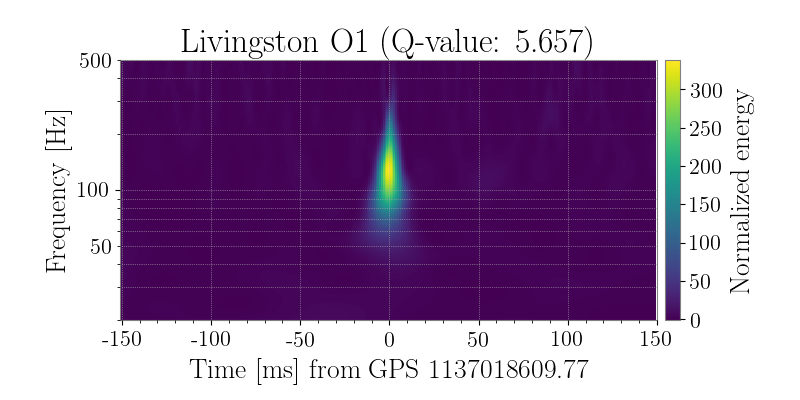
\includegraphics[width=1\linewidth]{normal_blip}
		\caption{Normal blip Q-transform}
		\label{fig:normal}
	\end{subfigure}
	\begin{subfigure}{.49\textwidth}
		\centering
		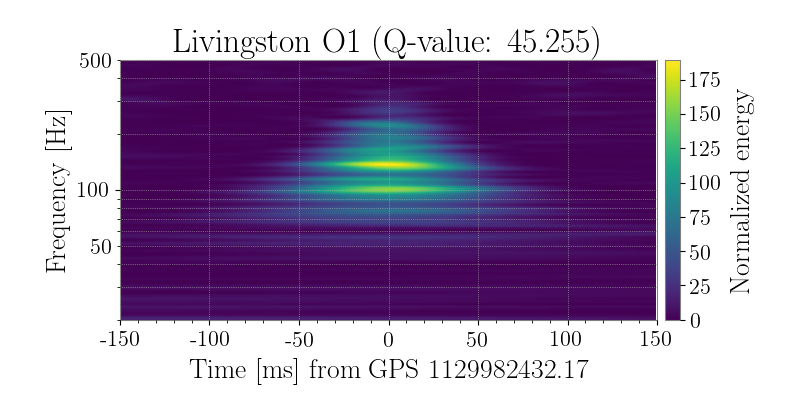
\includegraphics[width=1\linewidth]{spread_blip}
		\caption{Spread blip Q-transform}
		\label{fig:spread}
	\end{subfigure}
	\begin{subfigure}{.49\textwidth}
		\centering
		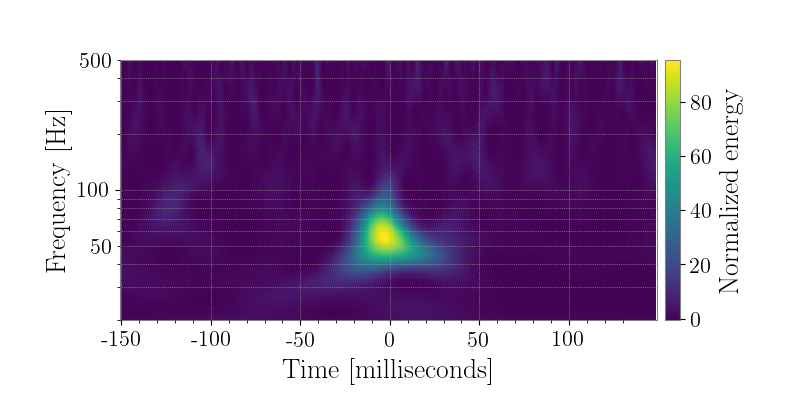
\includegraphics[width=1\linewidth]{dot_blip}
		\caption{Dot blip Q-transform}
		\label{fig:dot}
	\end{subfigure}
	\begin{subfigure}{.49\textwidth}
		\centering
		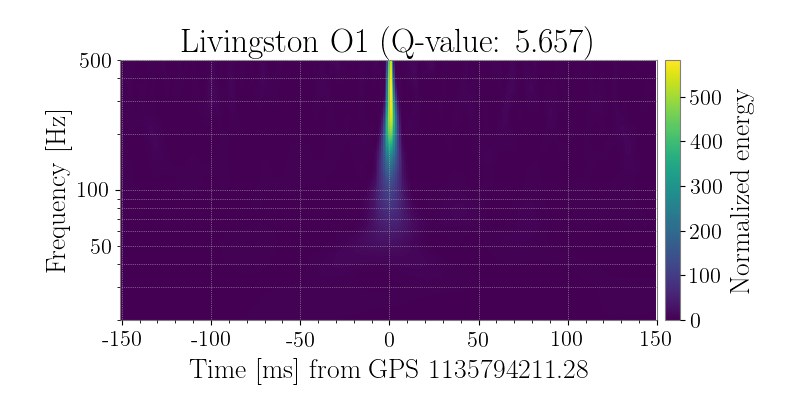
\includegraphics[width=1\linewidth]{stick_blip}
		\caption{Stick blip Q-transform}
		\label{fig:stick}
	\end{subfigure}
	\caption{Four different types of blip glitches from Livingston O1 in Q-transform spectrograms, all with the same time duration of 0.30 seconds, cropped from 30 seconds of transformed strain data. The Q-value calculated by GWpy is 5.65 for all but the spread blip (45.25). Note that the energy scale is different for each blip.}
	\label{fig:q_transforms}
\end{figure}

After discovering these differing forms in the Q-transforms, and plotting about 100 more Q-transforms, I looked at the existing GravitySpy spectrograms in LigoDV-Web of a specific blip from each of the four possible sub-classifications to determine the legitimacy of my assumptions, the results of which are in Figure \ref{fig:comparison} on page \pageref{fig:comparison}. (Note: Any future mention of a "spectrogram" refers to GravitySpy's spectrograms, and any future mention of a "Q-transform" refers to my own short-duration spectrograms.)

\begin{figure}[h!]
	\centering
	\begin{subfigure}[t]{.7\textwidth}
		\centering
		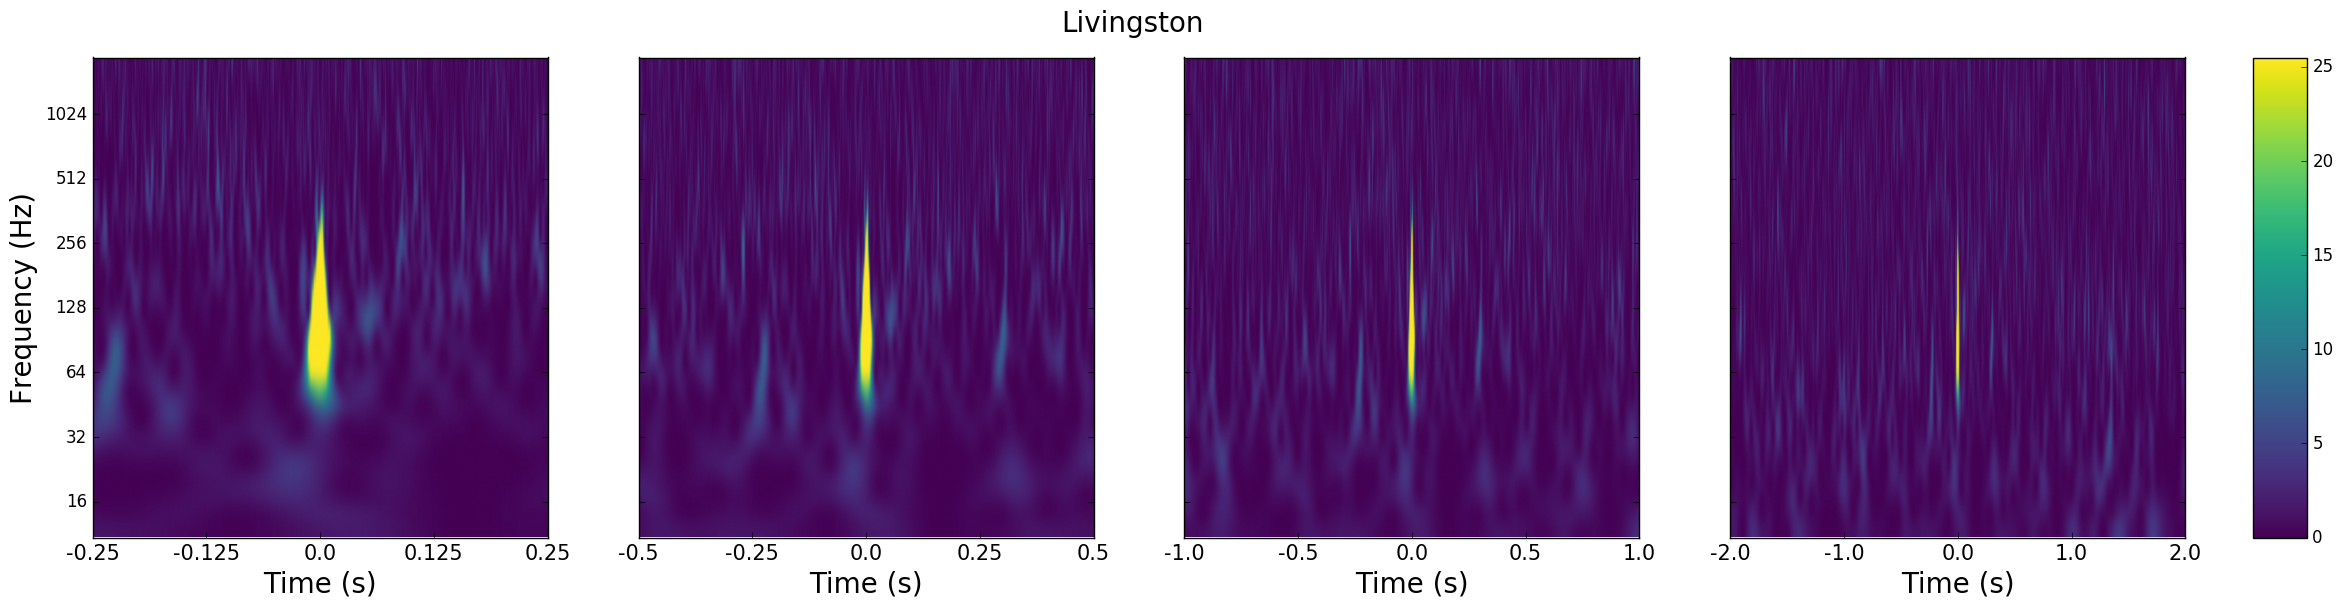
\includegraphics[width=.9\linewidth]{normal_blip_spect}
		\caption{Normal blip spectrograms}
		\label{fig:normal_s}
	\end{subfigure}
	\begin{subfigure}[t]{.29\textwidth}
		\centering
		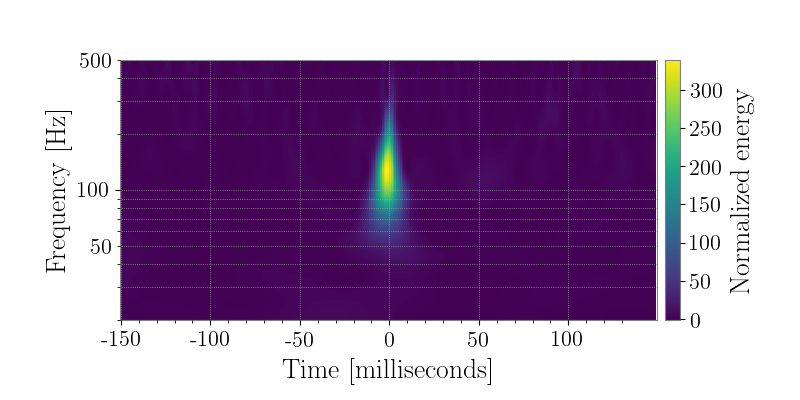
\includegraphics[width=1.1\linewidth]{normal_blip2}
		\caption{Normal blip Q-transform}
		\label{fig:normal_q}
	\end{subfigure}
	\begin{subfigure}[t]{.7\textwidth}
		\centering
		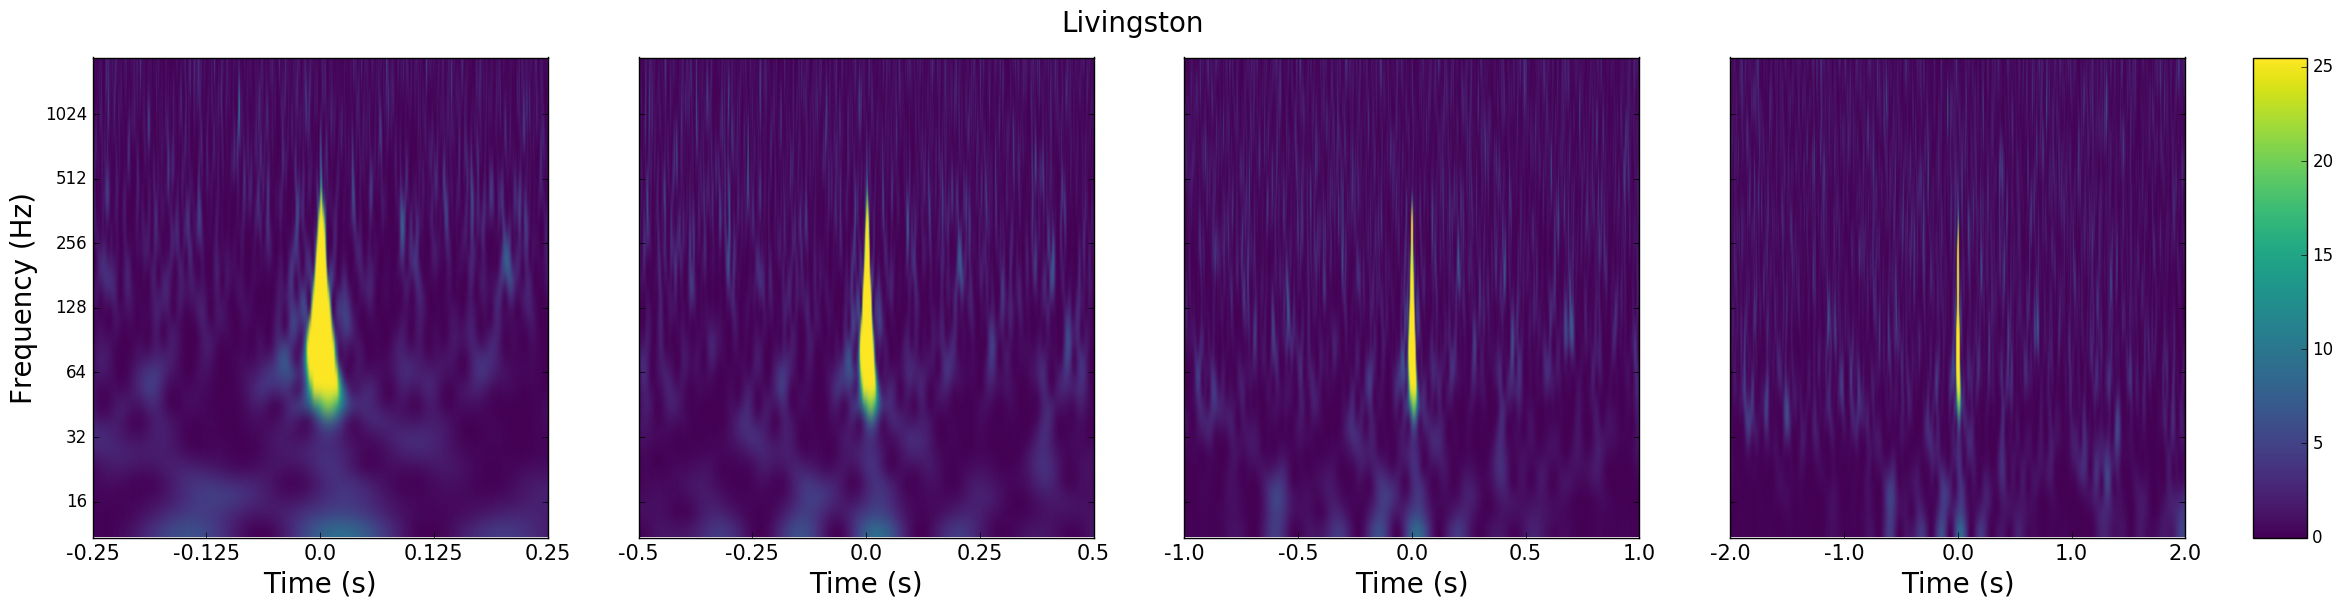
\includegraphics[width=.9\linewidth]{spread_blip_spect}
		\caption{Spread blip spectrograms}
		\label{fig:spread_s}
	\end{subfigure}
	\begin{subfigure}[t]{.29\textwidth}
		\centering
		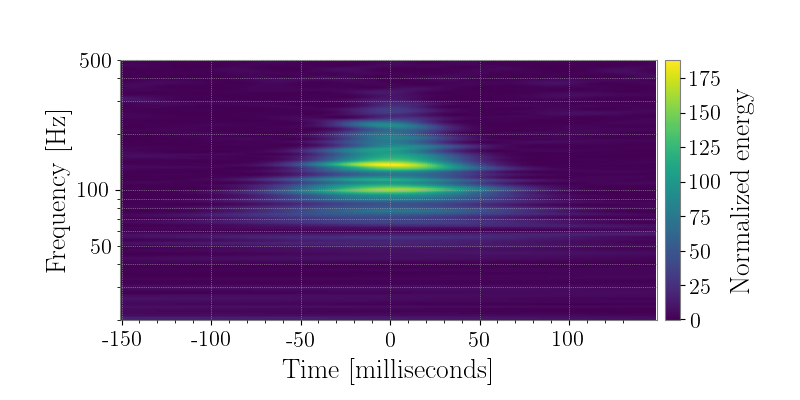
\includegraphics[width=1.1\linewidth]{spread_blip2}
		\caption{Spread blip Q-transform}
		\label{fig:spread_q}
	\end{subfigure}
	\begin{subfigure}[t]{.7\textwidth}
		\centering
		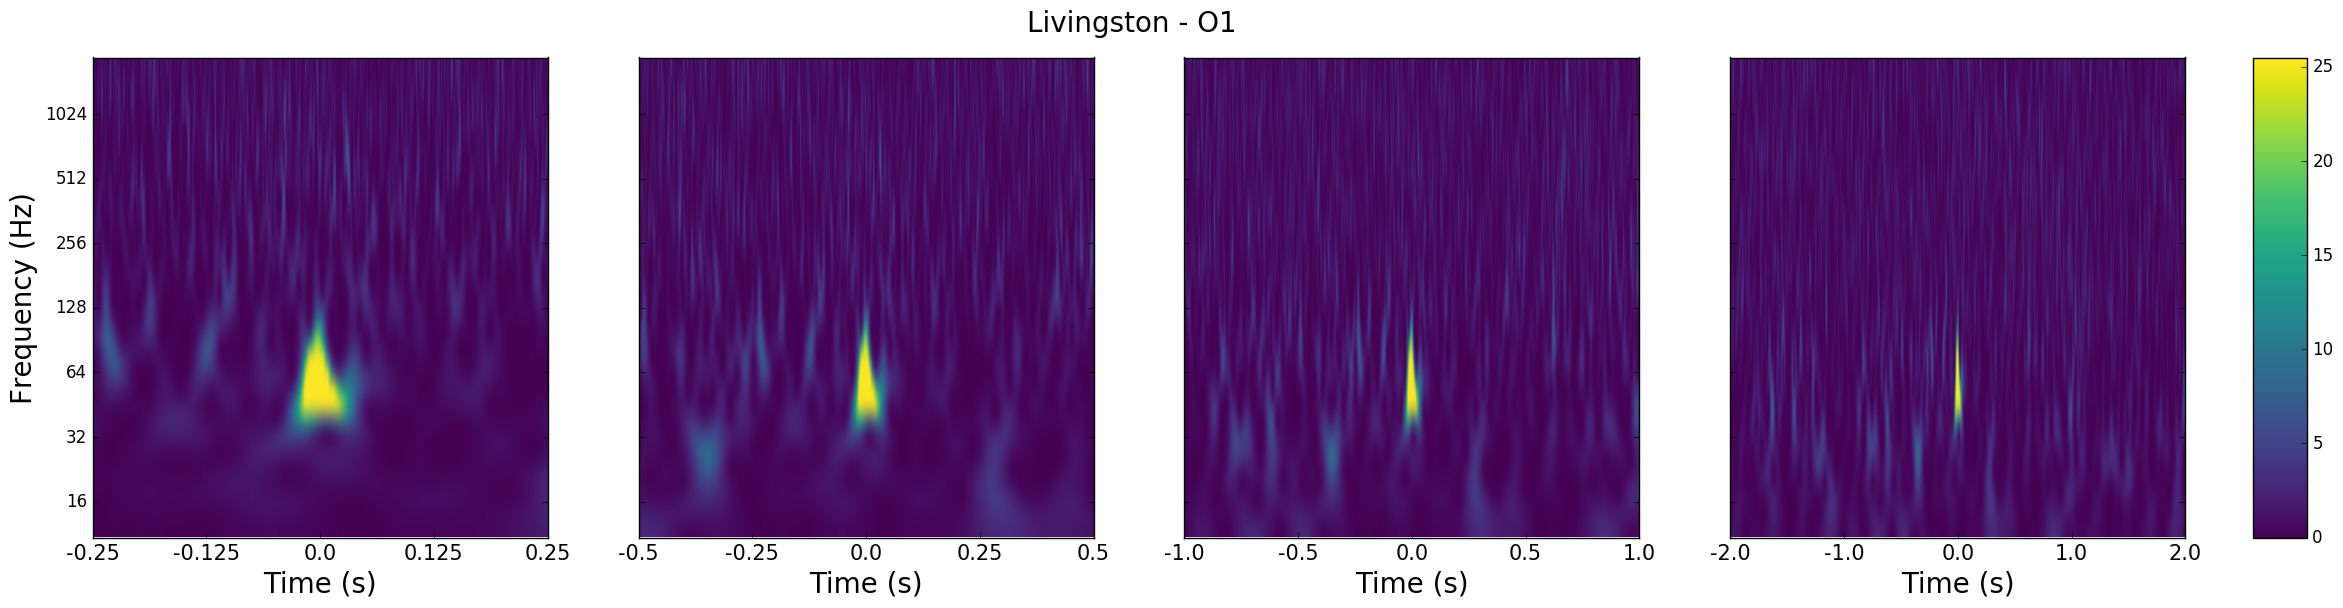
\includegraphics[width=.9\linewidth]{dot_blip_spect}
		\caption{Dot blip spectrograms}
		\label{fig:dot_s}
	\end{subfigure}
	\begin{subfigure}[t]{.29\textwidth}
		\centering
		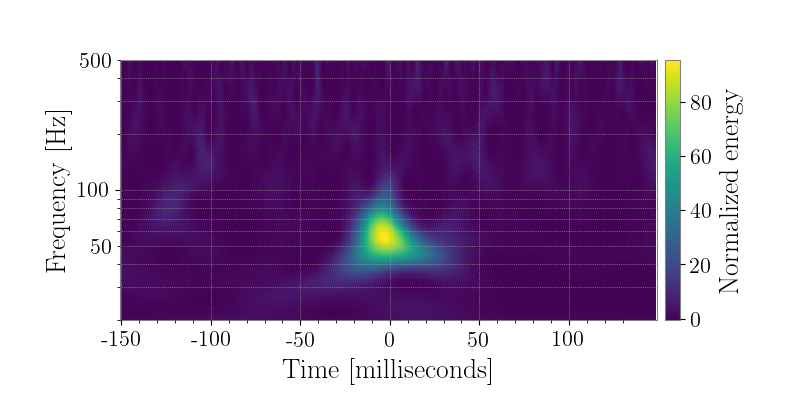
\includegraphics[width=1.1\linewidth]{dot_blip2}
		\caption{Dot blip Q-transform}
		\label{fig:dot_q}
	\end{subfigure}
	\begin{subfigure}[t]{.7\textwidth}
		\centering
		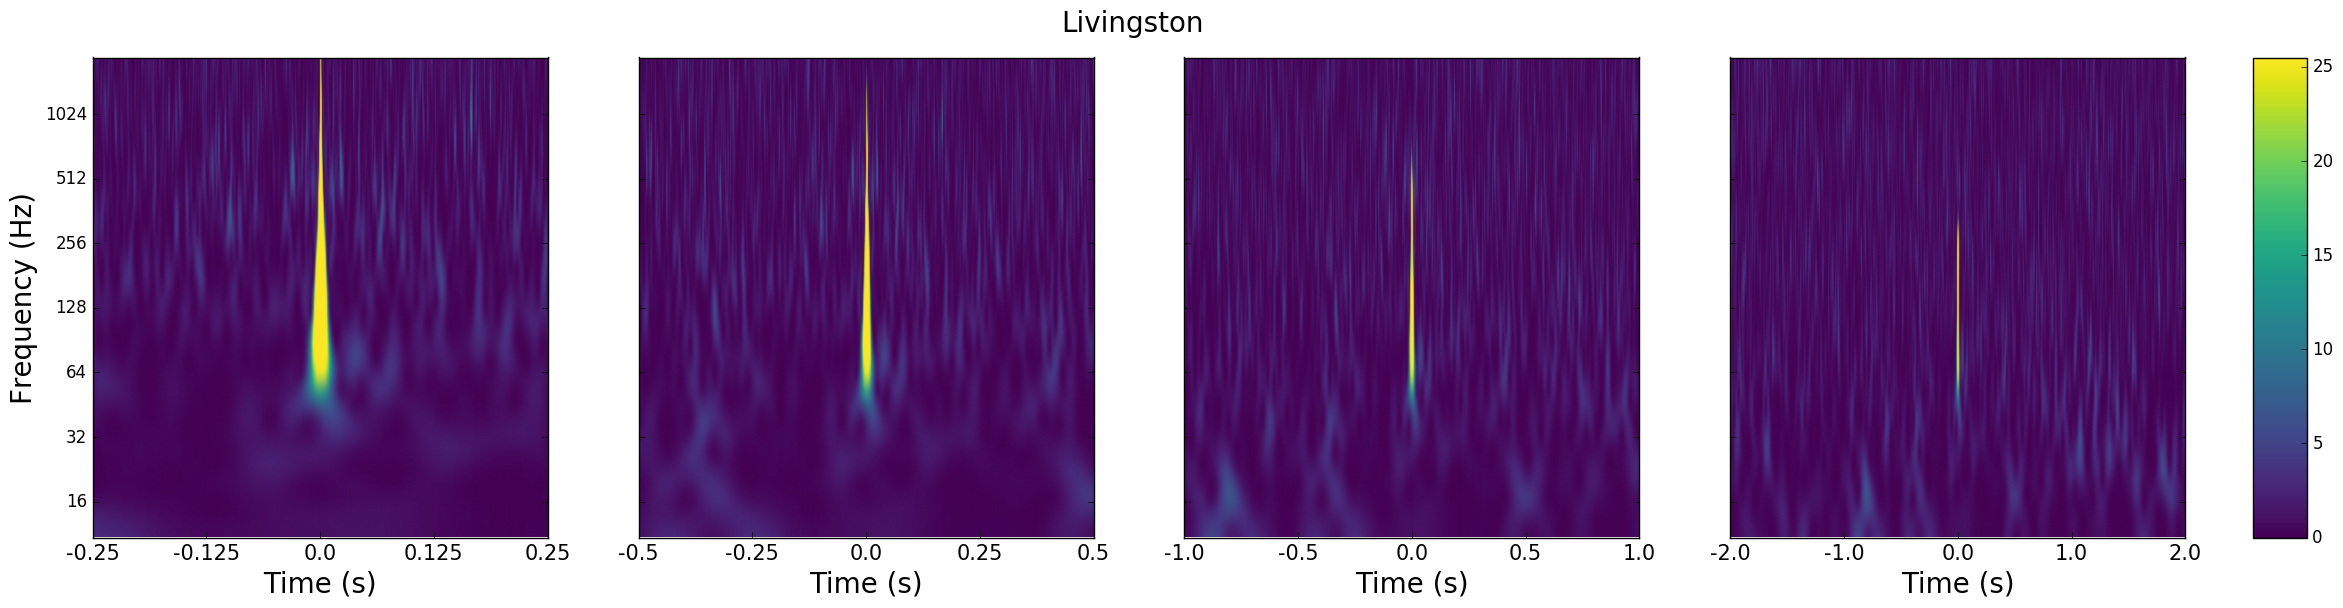
\includegraphics[width=.9\linewidth]{stick_blip_spect}
		\caption{Stick blip spectrograms}
		\label{fig:stick_s}
	\end{subfigure}
	\begin{subfigure}[t]{.29\textwidth}
		\centering
		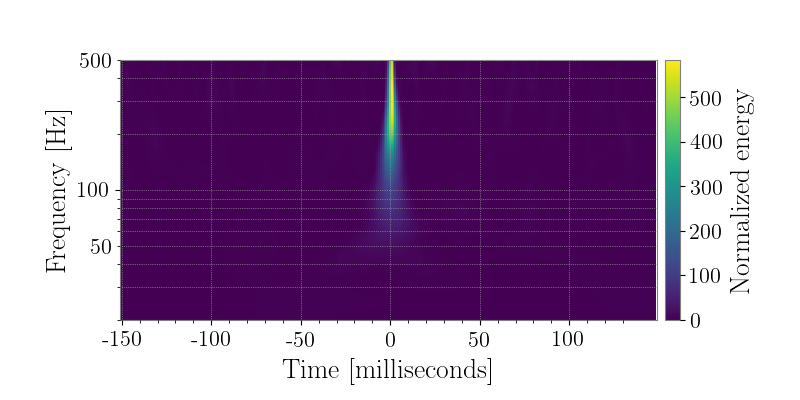
\includegraphics[width=1.1\linewidth]{stick_blip2}
		\caption{Stick blip Q-transform}
		\label{fig:stick_q}
	\end{subfigure}
	\caption{A comparison between GravitySpy spectrograms of four different blip glitches on the left and the corresponding short-duration Q-transform of the same blip glitches on the right. The spectrogram images come from LigoDV-Web, with time durations from left to right of 0.5 seconds, 1.0 seconds, 2.0 seconds, and 4.0 seconds. The Q-transform images were created from my Python script, cropped from 30 seconds of transformed data down to 0.30 seconds. The top row is a normal blip, the second row is a spread blip, the third a dot blip, and a stick blip on the bottom. Although the spectrograms of the different blips are somewhat distinguishable from one another, the Q-transforms reveal that these blip glitches may have fundamental differences.}
	\label{fig:comparison}
\end{figure}

The most striking difference between the spectrograms and the Q-transforms is in the images for the spread blip. The spectrograms from the normal blip and the spread blip, Figures \ref{fig:normal_s} and \ref{fig:spread_s}, appear to be almost exactly the same, but while the normal blip's Q-transform (Figure \ref{fig:normal_q}) has the same shape as its spectrogram, hence the name "normal," the spread blip's Q-transform (Figure \ref{fig:spread_s}) "spreads" outward with distinct horizontal lines. These horizontal lines (which are essentially frequency bins) initially suggest that the duration of a spread blip is longer than the rest of the blips and therefore it needs more data than 30 seconds for a clear Q-transform. Additionally, the much larger Q-value for the spread blip (45.25) is an immediate red flag and could suggest a problem with the transform.

The dot blip, on the other hand, has no red flags and looks like a legitimate sub-classification. The dot's Q-transform (Figure \ref{fig:dot_q}) has a distinct round shape at a relatively low frequency compared to the other blips. Dot blips also appear to have a slightly longer duration compared to other blips. The spectrogram of the dot blip (Figure \ref{fig:dot_s}) is also easily distinguishable from the others, with a much smaller frequency range and an almost triangle-like shape. This is an example of a possible distinguishable classification of glitch that GravitySpy groups in with blips, as mentioned in section \ref{introduction}. Since a dot blip can be identified on GravitySpy's spectrogram, it is highly possible that it could be easily classified apart from other blip glitches by GravitySpy. 

The stick blip also seems to be different than a normal blip. Its spectrogram (Figure \ref{fig:stick_s}) is only slightly skinnier than that of a normal blip, with a slightly longer upward tail. However, the Q-transform (Figure \ref{fig:stick_q}) reveals that a stick blip is at a significantly higher frequency than a normal blip. Even if the stick blip is the same shape as a normal blip, the higher frequency sets it apart, especially compared to dot blips.

This comparison between GravitySpy's spectrograms and my own Q-transforms validates GravitySpy's ability to classify similar images. The four shapes I found in the Q-transforms do not appear to be mis-classified, they simply have characteristics that cannot be discerned from GravitySpy's specific type of spectrogram. 

\subsection{Further Investigation into O2 and Hanford Blips} \label{O2}

Before delving into possible characteristics that could separate the types of blips I had found, I wanted to clear up the spread blip's Q-transform and see whether the same variety of shapes from my findings in O1 Livingston blips are present in O2 and at Hanford.

I attempted to condense the spread blips by creating another two Q-transforms for each spread blip using the surrounding 40 seconds and 60 seconds of data, rather than my original 30 seconds. I speculated that the image wasn't clear due to the signal having a longer duration compared to other blips. However, the exact same spread effect occurred for all of the known spread blips for both widened time domains. I went the other direction and reduced amount of surrounding to 20 seconds, which could indicate a problem with the internal whitening that occurs to create the spectrogram of the transform, rather than a signal duration problem. Fortunately, this shortening of the domain cleared the images and we could see the actual shapes of the spread blips, one example of which is in Figure \ref{fig:spread_ex} on page \pageref{fig:spread_ex}.

\begin{figure}[h!]
	\centering
	\begin{subfigure}{.49\textwidth}
		\centering
		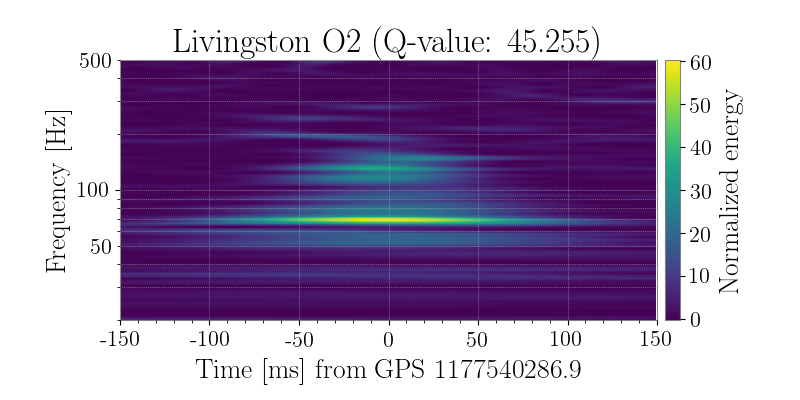
\includegraphics[width=1\linewidth]{spread_ex_30s}
		\caption{Spread blip with 30 second domain}
		\label{fig:spread_30}
	\end{subfigure}
	\begin{subfigure}{.49\textwidth}
		\centering
		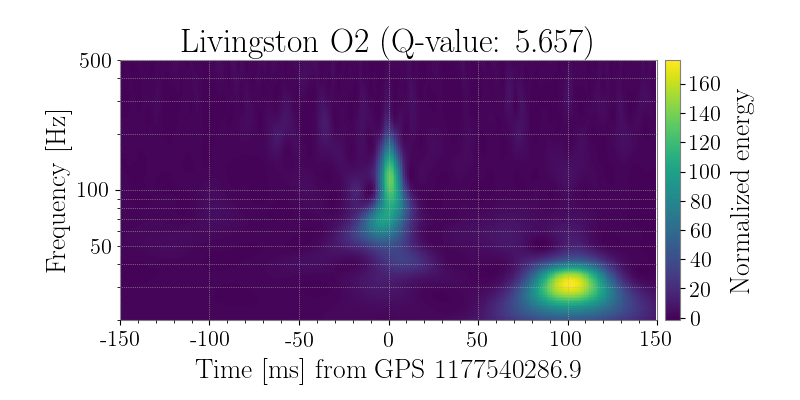
\includegraphics[width=1\linewidth]{spread_ex_20s}
		\caption{Spread blip with 20 second domain}
		\label{fig:spread_20}
	\end{subfigure}
	\caption{A blip glitch from Livingston O2 with two different amounts of surrounding data, both cropped back down to 0.3 seconds. This blip is called a double blip due to its secondary signal around 100 ms away from the center signal.}
	\label{fig:spread_ex}
\end{figure}

The change in amount of data gets rid of the spreading effect and brought the Q-value back down to the common blip Q-value of 5.65. It would appear that the original time domain parameter of the Q-transform was simply obscuring the image, but the Q-value in the original spread image is still suspicious. Although changing the amount of data to get rid of the spreading effect in my Q-transforms is good enough for the purposes of this project, the reason behind this spreading is unknown and could be a future point of investigation. Using this quick fix, most of the spreads condensed down to dots, normals, and sticks. The spread blip from Figures \ref{fig:q_transforms} and \ref{fig:comparison} turned out to be a normal blip, explaining why the spectrogram of the normal blip was so similar to that of the spread blip in Figure \ref{fig:comparison}. However, a few spreads did not fit into the three initial possible sub-classes, including a couple that appear to contain two different signals within 100 milliseconds of each other, such as Figure \ref{fig:spread_20}, which I call a double-blip. 

Now knowing that 20 seconds is a more consistent parameter for the Q-transform than 30 seconds, and also knowing that there was a large possibility for other types of blips beyond dots, normals, and sticks, I plotted and classified around 150 blip glitches from Hanford O2 and about 100 blip glitches from Livingston O2. I found six major shapes of blips, all of which are at both detectors, as shown in Figure \ref{fig:six} on page \pageref{fig:six}. The dot, stick, and normal are still there, but I also found double-blips, snitches (named for the Golden Snitch from \textit{Harry Potter}), and hats (named for the Sorting Hat from \textit{Harry Potter}). I also found a decent amount of individual unknown shapes that did not fit into the six classes. In this project, the focus was more on shapes that consistently showed up in both detectors, so the small number of unknown blips were largely overlooked for the rest of the project because they have a small effect on the amount of transient noise caused by blips.

\begin{figure}[h!]
	\centering
	\begin{subfigure}{.49\textwidth}
		\centering
		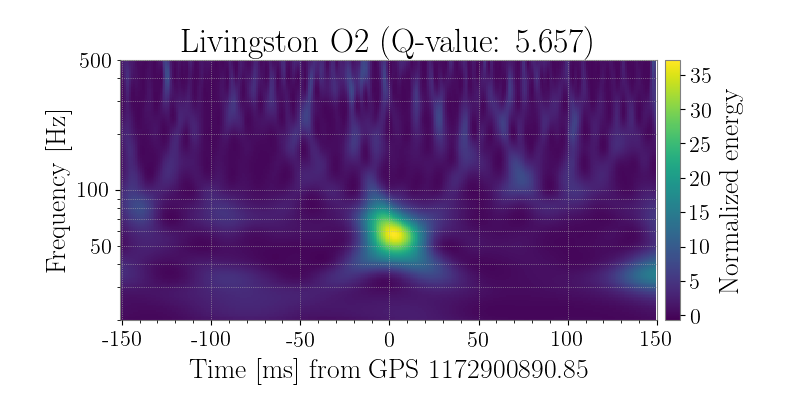
\includegraphics[width=1\linewidth]{dot_O2}
		\caption{Dot blip}
		\label{fig:dot_O2}
	\end{subfigure}
	\begin{subfigure}{.49\textwidth}
		\centering
		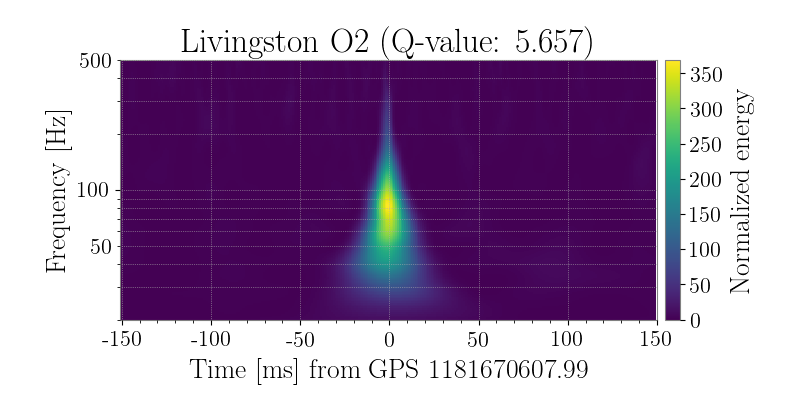
\includegraphics[width=1\linewidth]{normal_O2}
		\caption{Normal blip}
		\label{fig:normal_O2}
	\end{subfigure}
	\begin{subfigure}{.49\textwidth}
		\centering
		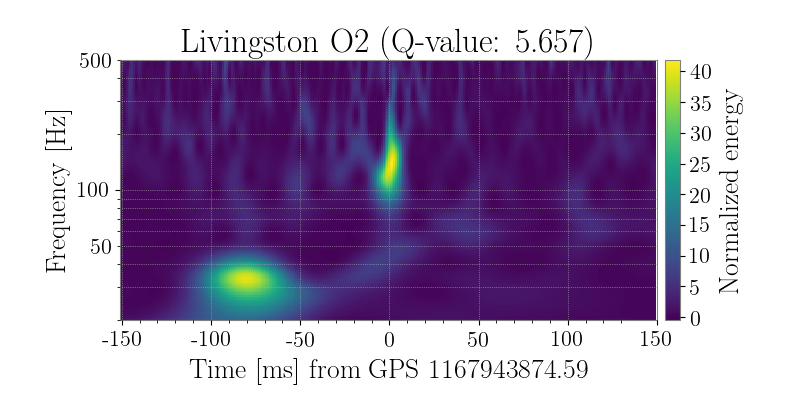
\includegraphics[width=1\linewidth]{double_O2}
		\caption{Double blip}
		\label{fig:double_O2}
	\end{subfigure}
	\begin{subfigure}{.49\textwidth}
		\centering
		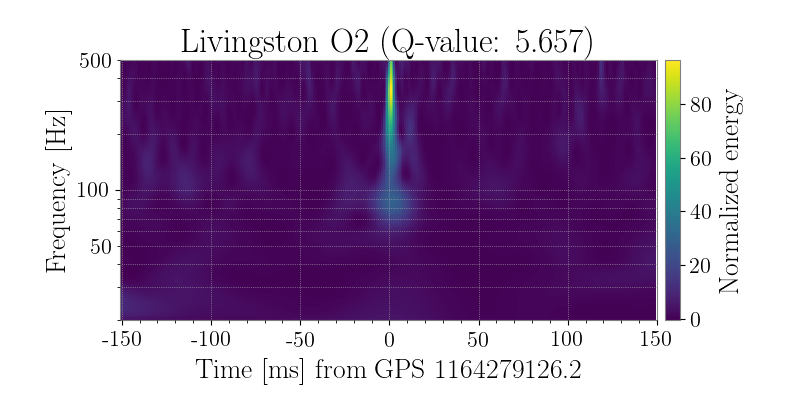
\includegraphics[width=1\linewidth]{stick_O2}
		\caption{Stick blip}
		\label{fig:stick_O2}
	\end{subfigure}
	\begin{subfigure}{.49\textwidth}
		\centering
		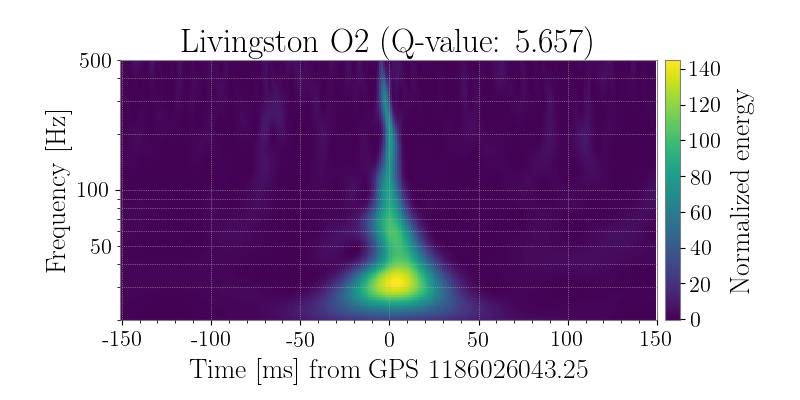
\includegraphics[width=1\linewidth]{hat_O2}
		\caption{Hat blip}
		\label{fig:hat_O2}
	\end{subfigure}
	\begin{subfigure}{.49\textwidth}
		\centering
		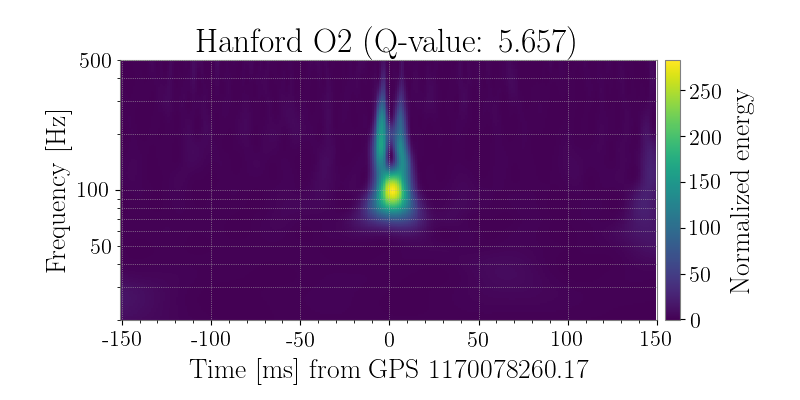
\includegraphics[width=1\linewidth]{snitch_O2}
		\caption{Snitch blip}
		\label{fig:snitch_O2}
	\end{subfigure}
	\caption{Six possible sub-classes of blips.}
	\label{fig:six}
\end{figure}

The variance in the background of each image is due to the relative energy of each blip. In this figure, the dot blip (Figure \ref{fig:dot_O2}) has a relatively low energy compared to the normal blip (Figure \ref{fig:normal_O2}), which is why the normal blip is so clear. However, I also found high energy dots and low energy normals in my image database. The double-blip, on the other hand, appears to always have relatively low energy, and it always has one low-frequency dot shape either about 100 ms before or after the mid-frequency, smaller duration signal that causes the Omicron trigger. It is unclear whether this is simply a coincidence, where two blips just so happen to be practically on top of each other, or if these are two connected signals in a cause-effect relationship, or if the low-frequency dot is simply a side effect of the whitening of the Q-transform. 

The hat blip, similar to the double-blip, is a complete mystery. The name comes from the wavy, squiggly nature of its shape, which is very different from the symmetry present in all the other types of blips (other than double-blips). The base of the hat in Figure \ref{fig:hat_O2} is at a fairly low frequency and all hats follow the general shape of a wavy top and a more spread-out, wavy bottom, but the bases of other hats are a slightly higher frequency. Hat blips are consistent in their general frequency range, which is low- to mid-frequency.

The last new blip is the snitch in Figure \ref{fig:snitch_O2}, which has two vertical, upward trails on either side of a round ball. Similar to other blip types, the snitch occurs at both high and low frequency. 

\section{Determining Distinguishable Characteristics of Possible Sub-Classifications of Blip Glitches} \label{plots}

Now that I had a fairly robust idea of the possible sub-classifications of blips, I searched for characteristics that could distinguish one type from another. The first step I took in finding specific attributes was to create a variety of histograms examining possible characteristics to find clusters of blips that might correspond to the six different types. I started with peak frequency and found a striking difference between the Livingston blips and the Hanford blips, as shown in Figure \ref{fig:combined} on page \pageref{fig:combined_peakf}. Since the scale is dependent on the Hanford blips, Figure \ref{fig:llo_peakf} shows the Livingston blips by themselves.

\begin{figure}[h!]
	\centering
	\begin{subfigure}{.49\textwidth}
		\centering
		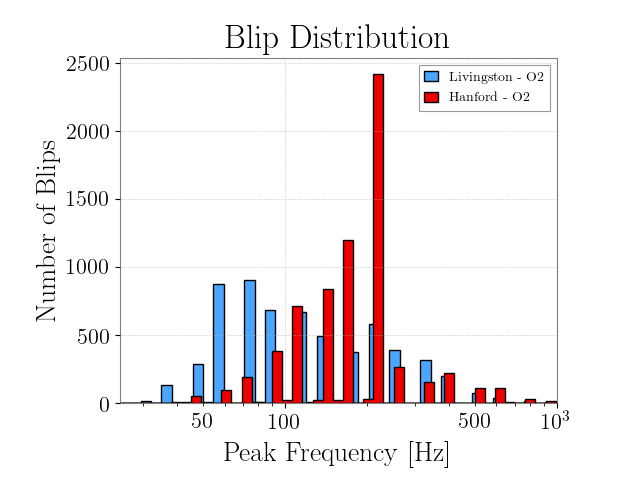
\includegraphics[width=1\linewidth]{combined_peakf}
		\caption{All O2 blips from Hanford and Livingston.}
		\label{fig:combined}
	\end{subfigure}
	\begin{subfigure}{.49\textwidth}
		\centering
		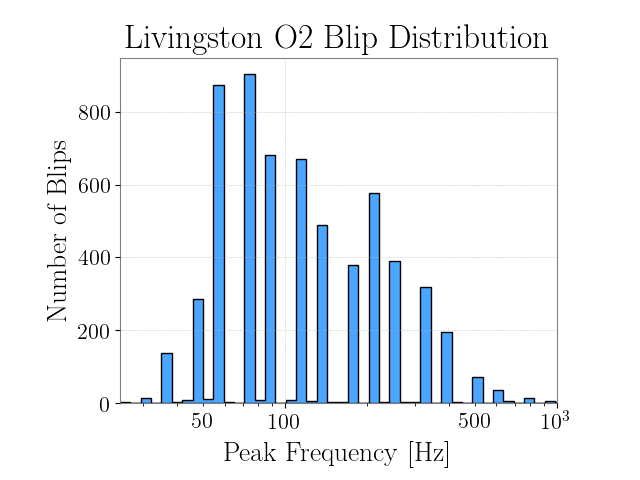
\includegraphics[width=1\linewidth]{llo_peakf}
		\caption{Livingston blips}
		\label{fig:llo_peakf}
	\end{subfigure}
	\caption{Peak frequency histograms for blips during O2.}
	\label{fig:combined_peakf}
\end{figure}

These histograms show a clear difference between the Livingston blips and the Hanford blips, which is somewhat surprising considering that all six blip shapes are found in both detectors. Most of the Hanford blips appear to have a peak frequency of 200 Hz, with a fairly steep dropoff on both sides of the 200 Hz spike. The Livingston blips, on the other hand, look to be more evenly spread out among the different frequencies, and there are considerably more low-frequency blips at Livingston. One possible explanation for this is that Livingston just happens to be more sensitive at low frequencies, but it could also be that the blips are simply different at different detectors.

To get a closer look at the Livingston blips and see if there is anything significant going on within Hanford's 200 Hz spike, I made 2D histograms plotting peak frequency versus SNR (signal to noise ratio) for each detector. Figure \ref{fig:hists_2d}  on page \pageref{fig:hists_2d} shows these histograms. Here, the differences between Livingston and Hanford are even more clear. For example, while Livingston's peak frequency distribution (Figure \ref{fig:llo_peakf}) does show a local maxima around 200 Hz, the 2D histogram of Livingston reveals that most of those blips have a low SNR, whereas a considerable amount of Hanford 200 Hz blips have a high SNR. 

\begin{figure}[h!]
	\centering
	\begin{subfigure}{.49\textwidth}
		\centering
		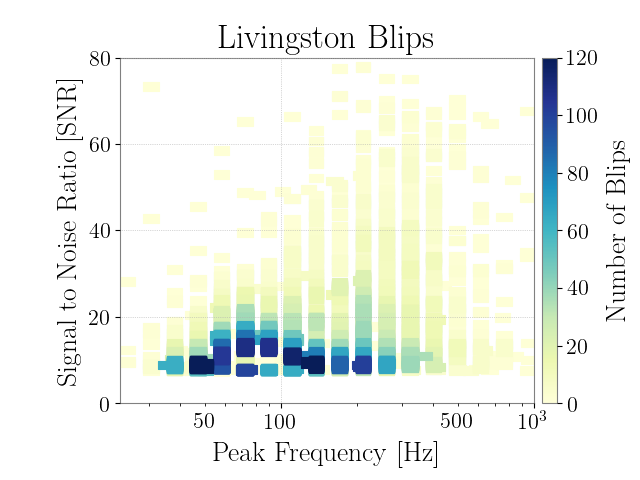
\includegraphics[width=1\linewidth]{llo_2d}
		\caption{Livingston 2D histogram}
		\label{fig:llo_2d}
	\end{subfigure}
	\begin{subfigure}{.49\textwidth}
		\centering
		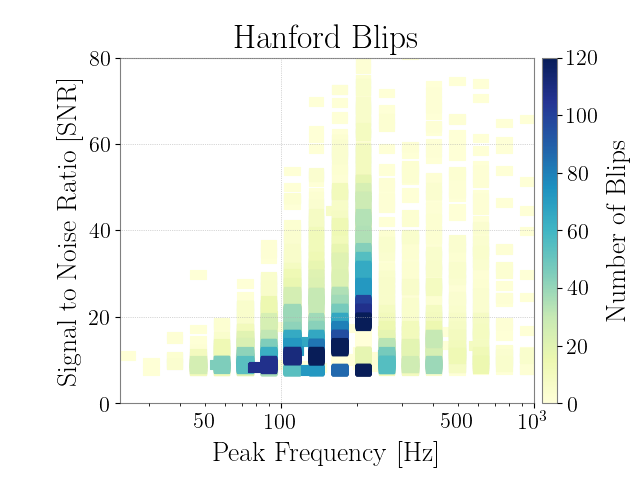
\includegraphics[width=1\linewidth]{lho_2d}
		\caption{Hanford 2D histogram}
		\label{fig:lho_2d}
	\end{subfigure}
	\caption{Peak frequency versus SNR 2D histograms of blips from O2.}
	\label{fig:hists_2d}
\end{figure}

Looking at the broader shape of each 2D histogram, both appear to have a clear arc shape over a range of frequencies, where an increase in frequency also increases the SNR, and then at even higher frequencies, the SNR decreases. At Livingston, it starts with low-SNR blips around 50 Hz and ends around 150 Hz. At Hanford, we can see the same general arc from about 80 Hz to the low-SNR blips at 200 Hz, but the high-SNR blips at 200 Hz are clearly separate from the arc. The similarity in the arcs from both detectors raise interesting hypotheses. For example, the blips at the start of each arc might be similar, even though the peak frequencies are different. 

Another data value that could be investigated is central frequency. Although it is similar to peak frequency, it might shed more light on the similarities between the Hanford and Livingston blips and the 200 Hz blips at Hanford. I created another two 2D histograms, one each for Hanford and Livingston, this time plotting central frequency versus peak frequency. The histograms are in Figure \ref{fig:central_hists} on page \pageref{fig:central_hists}.

\begin{figure}[h!]
	\centering
	\begin{subfigure}{.49\textwidth}
		\centering
		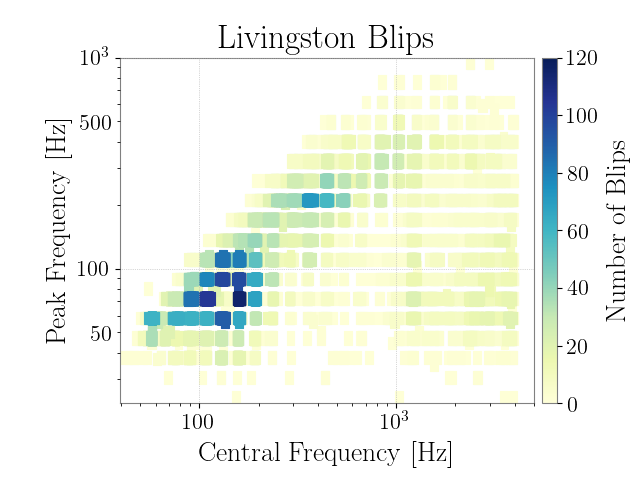
\includegraphics[width=1\linewidth]{llo_peak_v_centr}
		\caption{Livingston 2D histogram}
		\label{fig:llo_centr}
	\end{subfigure}
	\begin{subfigure}{.49\textwidth}
		\centering
		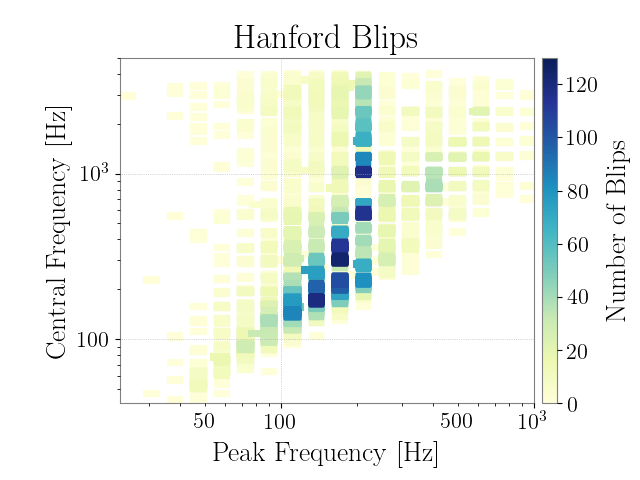
\includegraphics[width=1\linewidth]{lho_peak_v_centr}
		\caption{Hanford 2D histogram}
		\label{fig:lho_centr}
	\end{subfigure}
	\caption{Peak frequency versus central frequency 2D histograms of blips from O2.}
	\label{fig:central_hists}
\end{figure}

In these histograms, any similarities between the two detectors dissolve away. The high-density bins at Livingston create a completely different overall shape than those at Hanford. One thing that is especially interesting is the 200 Hz peak at Livingston, which has the highest-density bin around 350 Hz central frequency, and at Hanford, 350 Hz is one of the few places along the 200 Hz peak frequency bin where there are hardly any blips. Additionally, the histogram of Hanford reveals at least three different clusters of blips within the 200 Hz peak. 

Every cluster on either the SNR or central frequency histograms has the possibility of corresponding to a certain shape in the Q-transform spectrogram. We can use neural networks to investigate these possible clusters and see if any of them have a correspondence to the six types of blips I identified in section \ref{O2}. 

\section{Neural Network Implementation}

At this point in the project, Neural Networks become more desirable than histograms and manual searching. We want to know if the six types of blips can be identified by a computer, not just one person looking at a couple hundred images. If a Neural Network can be used to find the differences between the types of blips, then we know that sub-classification is possible and can be implemented in GravitySpy to classify all blips, bringing us a huge step forward in finding a source. I implemented the Neural Networks through Keras\footnote{\href{https://keras.io}{Keras documentation}}, using a TensorFlow\footnote{\href{https://www.tensorflow.org}{TensorFlow website}} backend.

\subsection{Building a Neural Network} \label{section:build_nn}

There are countless ways to build and implement a Neural Network. The first step is deciding what type of learning we want: supervised learning, reinforcement learning, or unsupervised learning. Reinforcement learning can almost immediately be discarded because it depends on a function to reward the program. Images cannot be easily translated into a function, so reinforcement learning is off the table. Supervised learning, on the other hand, is easy to implement and has a clear method for knowing whether the neural network is doing well or not. Unfortunately, supervised learning requires a large dataset of pre-labeled inputs, which we do not have. The ideal technique is therefore unsupervised learning, which doesn't need pre-set labels and trains using any metric that we want. However, unsupervised learning is extremely complex and the success of an unsupervised network is difficult to gauge. I ended up implementing both supervised and unsupervised learning neural networks\textemdash sections \ref{section:sup} and \ref{section:unsup} explain the types of networks and the reasons for using them in more depth.

The next step in creating a neural network is deciding the type of layers to put in the network. Since I want my input set to consist of images, I used Convolutional Neural Networks (CNNs) in both the supervised and unsupervised models. CNNs are better for images than a normal dense layer because they take all the surrounding points into consideration. Each image is stored as a multi-dimensional array, but normal dense layers can only interpret a single array, and can therefore only see pixels that are horizontally next to each other. CNNs take in multi-dimensional arrays as input and use all the surrounding pixels to learn about the image. A more technical explanation is that CNNs are actually CNN layers paired with pooling and up-sampling layers to manipulate the images in different ways. The CNN reshapes the image somehow, meaning that a 50x100 array (pixel image) could get converted to a 25x200 array. Pooling layers look at groups of pixels to create a smaller image. For example, imagine a square spilt into four colored squares, each colored square representing a pixel. The pooling layer will look at the four squares, find the average color, and create a new image with only one pixel where the four pixels used to be. Pooling down-converts an image, for example turning a 50x100 image into a 25x50 image. Upsampling layers are the opposite of pooling, this time extrapolating four pixels from one starting pixel. All three types of layers have weights associated with them, so each time through training, the effect of each layer changes slightly. The combination of these three types of layers create a Convolutional Neural Network.

The last thing to do before creating the neural networks themselves is to create the input dataset, in this case the images. I created a database of Q-transform spectrograms of all the blips from Hanford and Livingston during O2. each image used a standardized amount of data (20 seconds) and was cropped down to a time domain of 0.22 seconds, which is a slightly smaller than previous images I had created. I left the energy colorbar to scale itself during the calculation, mostly because the disparity between blips with low energy and blips with high energy is so drastic that the shapes become difficult to distinguish with a standardized energy scale. An example of the images in the database is in Figure \ref{fig:image}. Since there are no axes or titles, the images are labeled with their GPS time and detector from their file names. This file labeling allows access to the images of specific blips, which is helpful for both supervised and unsupervised learning.

\begin{figure}[h!]
	\centering
	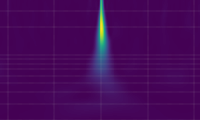
\includegraphics[width=.4\linewidth]{image}
	\caption{An example of the 120 x 200 images in the database used as input into neural networks.}
	\label{fig:image}
\end{figure}

\subsection{Supervised Learning Neural Network} \label{section:sup}

The goal of my supervised learning neural networks is to see whether specific attributes of blips create clusters. We can label specific blips based on their Omicron trigger values, such as peak frequency or bandwidth, and then evaluate the correlation based on the accuracy of the trained neural network. For example, I can label all the 200 Hz blips from Livingston with a "1," and label all the 200 Hz blips from Hanford with a "0," and see if the neural network can distinguish which images are from which detector. A supervised network is trained on a subset of the labeled inputs, usually around 80-90 \%, leaving the rest for testing. If the Hanford 200 Hz blips are fundamentally different than the ones at Livingston (which would be assumed, based on the histogram plots in section \ref{plots}), the neural network should have a high accuracy and "classify" the blips easily.

The example above is a case of binary classification, but we can create a neural network with as many classes as we want. Additionally, most neural networks have one input, but we can also create a two-input neural network that takes in both images and auxiliary data from the omicron trigger. As a result, I created four neural networks templates: one-input binary, two-input binary, one-input multi-class, and two-input multi-class. All four have almost exactly the same network of layers, but since they all have different uses, it is easy to implement different ideas. A condensed version of the layers in both of the two-input neural networks is in Figure \ref{fig:sup_condensed}. The only difference between the two-input CNN and the one-input CNN is that the \texttt{Flatten()} layer goes straight to the first \texttt{Dense()} layer with only one input. To make this network multi-class instead of binary, the output shape of the \texttt{main\_output} layer is changed from 1 to the number of classes, and the loss function is changed from \texttt{binary\_crossentropy} to \texttt{categorical\_crossentropy}. All layers other than the output layer in the supervised networks used the \texttt{relu} activation function, which was chosen in part because it is commonly used to to its advantages over \texttt{sigmoid} functions, and in part because it appeared to result in higher accuracy compared to other common functions\footnote{Other tried functions include \texttt{sigmoid}, \texttt{tanh}, \texttt{selu}, and \texttt{elu}. All functions either produced the same accuracies as \texttt{relu} or worse.}. For binary classification, the output activation function was \texttt{sigmoid}, and for multi-classification, the activation was \texttt{softmax}.

\begin{figure}[h!]
	\centering
	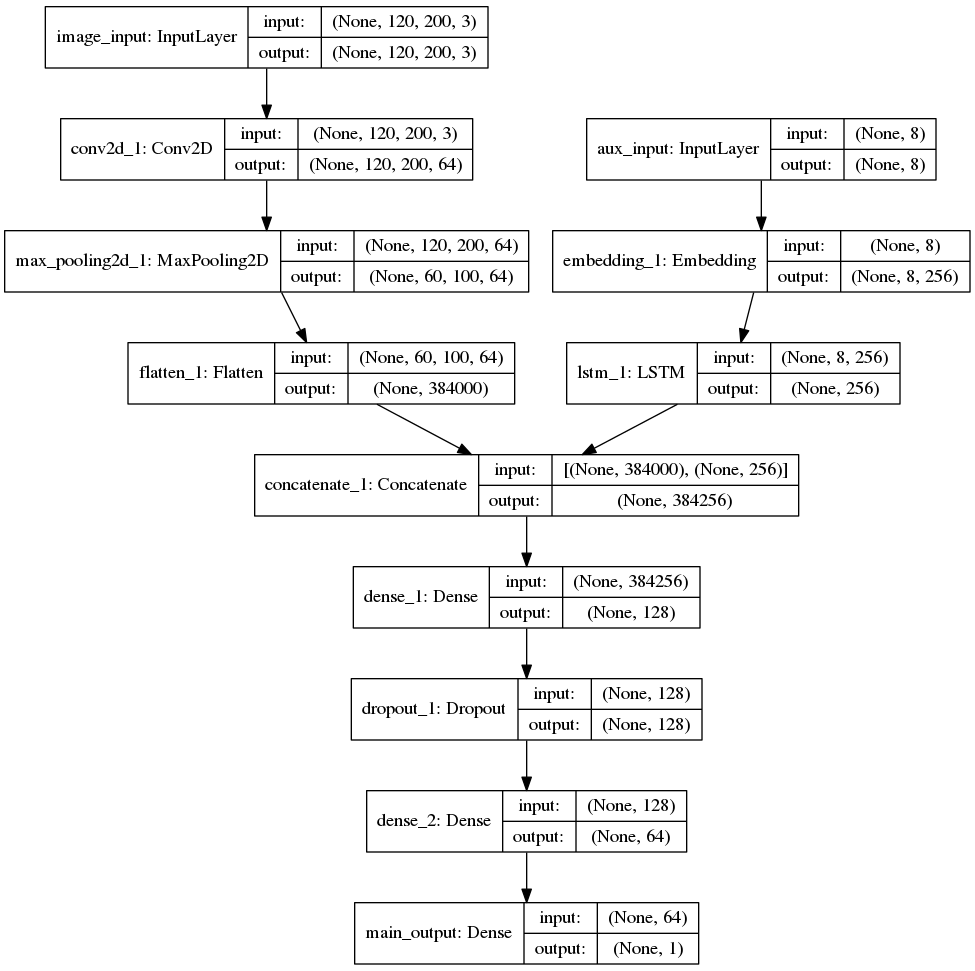
\includegraphics[width=.5\linewidth]{sup_condensed}
	\caption{Condensed version of my two-input Convolutional NN. There are additional \texttt{Conv2D()} and \texttt{MaxPooling2D()} layers between the \texttt{Input()} layer and the \texttt{Flatten()} layer, and an additional \texttt{Dropout()} and \texttt{Dense()} layer before the \texttt{main\_output}.}
	\label{fig:sup_condensed}
\end{figure}

The auxiliary input that went into the two-input neural networks consists of about 6-12 omicron data values, including but not limited to q-value, confidence, SNR, bandwidth, duration, interferometer, and image status. The shape of the auxiliary input, meaning the number of values in each input set, as well as the content, varies depending on what "classes" the neural network is looking at. Going back to the earlier example about distinguishing Livingston 200 Hz blips from Hanford 200 Hz blips, that auxiliary input would not include the interferometer or the peak frequency of each blip. 

Although adding auxiliary input seems helpful because it gives the neural networks more information, the performance difference between one-input neural networks and two-input neural networks is practically non-existent. Using images by themselves is exactly the same as using images along with auxiliary data. This is consistent with GravitySpy, which is directly dependent on images. The auxiliary data is not robust enough to aid in classification, both in GravitySpy's glitch classification and this project's sub-classification of blips. As a result, I mostly use the one-input neural networks. A summary of the different supervised learning neural networks that I ran and their conclusions and implications is in the next section.

\subsubsection{Results of Supervised Network}

As mentioned in the previous section, I first started with both one-input and two-input neural networks, then stopped using the two-input networks when it was clear that the auxiliary input had no impact on the neural networks. A summary of the networks and their end results are in Table \ref{table:1}, with more detailed descriptions of each network to follow. Although this table doesn't include every single neural network that I ran, all other networks were inconclusive due to reasons similar to those explained in the inconclusive networks described below. The most relevant of all the supervised networks are highlighted in the table.

%black, blue, brown, cyan, darkgray, gray, green, lightgray, lime, magenta, olive, orange, pink, purple, red, teal, violet, white, yellow

\begin{table}[h!]
\centering
\begin{tabular}{||c c c c c c||} 
 \hline
 NN & Input & Classes & (Training, Testing) & End Loss & Test Accuracy \\ [0.5ex] 
 \hline\hline
 1 & One-input & Binary & (2461,410) & 0.4483 & 0.1585 \\
 \multirow{2}{*}{\hfil 2} & One-input & Binary & (573,63) & 0.5310 & 0.8571 \\ 
  & Two-input & Binary & (573,63) & 0.5288 & 0.8571 \\ 
  \multirow{2}{*}{\hfil 3} & One-input & Binary & (1178,130) & 0.6792 & 0.3540 \\ 
  & Two-input & Binary & (1178,130) & 0.6824 & 0.3540 \\
 \rowcolor{pink}
  & One-input & Binary & (521,57) & 0.6640 & 0.0877 \\
  \rowcolor{pink}
 \multirow{-2}{*}{\hfil \hyperlink{binary}{4}}& Two-input & Binary & (521,57) & 0.6643 & 0.0702 \\
 5 & One-input & Binary & (1196,132) & 0.6956 & 0.1288 \\
 6 & One-input & Binary & (369,41) & 0.6255 & 0.7317 \\
 7 & One-input & Binary & (938,104) & 0.6935 & 0.4808 \\
 \rowcolor{pink}
 \hyperlink{multi}{8} & One-input & Multi & (1089,181) & 1.4652 & 0.3923 \\
 9 & One-input & Multi & (1472,245) & 1.2798 & 0.3224 \\
 \hline
\end{tabular}
\caption{Summary of supervised networks used. Networks that can give the most useful information have large datasets, low end loss, and test accuracy close to 0 or 1. Note that comparing the loss between binary and multi-class networks is insignificant because of the different loss functions. The most important column is the test accuracy, which is the percentage of test data that was correctly predicted by the trained neural network. A test accuracy close to 1 corresponds to a strong difference between the classes, and a test accuracy close to 0 means the network was not able to train itself properly. }
\label{table:1}
\end{table}

Although each network is comprised of the same set of layers, as explained in the previous section, each input is labeled differently with the aim of finding characteristics that correspond to actual differences in the shape of the images. The binary classification networks were based on the high-density bins in Figures \ref{fig:hists_2d} and \ref{fig:central_hists}. The details corresponding to the numbered networks in Table \ref{table:1} follow. 
\begin{enumerate}

	\item Peak frequency 200-220 Hz blips from both detectors
	\begin{itemize}
		\item Class 0: Hanford blips
		\item Class 1: Livingston blips
	\end{itemize} This neural network aimed to see if the Livingston blips are fundamentally different than the Hanford blips despite both detectors containing the same shapes of blips. The combination of the low end loss and low test accuracy suggests that the disparity between the amount of 200 Hz blips at Hanford (2405 in total) compared to Livingston (470 in total) is affecting the neural network's ability to train. Since there are so few Livingston images, the majority of the training set is guaranteed to be from Hanford. So, the results from this neural network (any any other networks with a large number disparity between groupings) cannot be reliable and are therefore inconclusive.

	\item Low-SNR blips from Hanford (Figure \ref{fig:lho_2d}). 	
	\begin{itemize}
		\item Class 0: Peak frequency between 80-100 Hz
		\item Class 1: Peak frequency between 200-220 Hz
	\end{itemize} As shown in Table \ref{table:1}, the one-input network and two-input network yielded the same test accuracy (0.8751), which is the first example of auxiliary input having little to no impact on the network. The test accuracy is high, meaning that the two groups appear to be distinguishable. However, the training set is rather small, at less than 600 images, so no conclusions can be made from this network alone.

	\item Hanford 200-220 Hz peak frequency (Figure \ref{fig:lho_2d}). 
	\begin{itemize}
		\item Class 0: SNR less than 10
		\item Class 1: SNR between 15-30
	\end{itemize} Due to the large, clear hole within the 200 Hz Hanford column in Figure \ref{fig:lho_2d}, the assumption going in was that this network would have a very high test accuracy. Unfortunately, both the one-input and two-input networks were about 35\% accurate, which gives an inconclusive result despite such a large input dataset.
	
	\item \hypertarget{binary}{Left-most bin} in Figures \ref{fig:llo_2d} and \ref{fig:lho_2d}.
	\begin{itemize}
		\item Class 0: Livingston blips with peak frequency between 40-50 Hz
		\item Class 1: Hanford blips with peak frequency between 80-100 Hz
	\end{itemize} Even though the dataset for this network is very small, the extremely low test accuracy is an immediate sign of interest. The neural network could not be trained to predict the class of practically any image. The initial assumption is that these two groups must consist of the same images, so it is impossible to determine which class each image belongs. Unfortunately, this assumption is naive, since if two classes were truly the same, the neural network should be about 50\%, the same as a coin flip. So, something else is preventing the neural network from correctly guessing the class of each test image. I investigated by looking at about 15 images from each class, and discovered that multiple types of images were in both groupings, specifically dots, hats, and normals. This is clearly the source of the extremely low test accuracy, because the neural network is trying to do binary classification on two groups that contain three different shapes of images. For example, a test image in the shape of a hat might be predicted to be from Hanford because there were slightly more hats at Hanford in the training set than at Livingston, but there is actually no reason for that particular hat to be from Hanford since there are hats in that specific bin at Livingston as well. Unfortunately, this means that a test accuracy close to zero is actually an indicator of a useless neural network, rather than an indicator of finding two groupings that are the same, which was my initial thought on the matter. 
	
	\item Next left-most bin in Figures \ref{fig:llo_2d} and \ref{fig:lho_2d}.
	\begin{itemize}
		\item Class 0: Livingston blips with peak frequency between 55-65 Hz
		\item Class 1: Hanford blips with peak frequency between 100-120 Hz
	\end{itemize} Similar to the previous neural network, this binary classification has an extremely low test accuracy. This network, on the other hand, had a very large training dataset, which means the results are more reliable than other input sets. However, the results are just as inconclusive as the last example due to the low test accuracy, and the images in each class similarly consist of dots, hats, and normals.

	\item Hanford 200-220 Hz peak frequency (Figure \ref{fig:lho_centr}). 
	\begin{itemize}
		\item Class 0: Central frequency between 500-600 Hz
		\item Class 1: Central frequency between 900-1100 Hz
	\end{itemize} Now moving on to the bins in the central frequency 2D histograms from Figure \ref{fig:central_hists}, this neural network is one of the first to have possible conclusive results, and it is an attempt at finding differences within the 200 Hz Hanford blips. The test accuracy is considerably higher than 50\% at 0.7317, but unfortunately the images from both groupings appear to be mostly sticks and high-frequency central frequencies. It is a strong possibility that the extremely small training dataset just so happened to throw off the accuracy from 50\% since the images don't appear to show any differences. 
	
	\item Central frequency 160-200 Hz from both detectors (Figure \ref{fig:central_hists})
	\begin{itemize}
		\item Class 0: Hanford blips
		\item Class 1: Livingston blips
	\end{itemize} The test accuracy for this network is the closest to 50\% out of all the supervised networks, suggesting that these two groupings are similar, and possibly only include a single shape. After examining some images in each grouping, it seems my assumptions about a binary supervised network with a test accuracy around 50\% are correct; almost all the images in both groupings are normals with a fairly high frequency. 
	
	\item \hypertarget{multi}{Self-labeled blips} from both Hanford and Livingston with no specific parameters
	\begin{itemize}
		\item 6 Classes: Dots, Hats, Normals, Snitches, Sticks, Doubles
	\end{itemize} Although I managed to create a reasonably-sized dataset of sub-class-labeled blips, multi-classification is difficult to even get to 50\% accuracy. If two of the classes are difficult to distinguish between, such as possibly hats and normals, the same result as in network \hyperlink{binary}{4} occurs for those classes, bringing down the overall effectiveness of the training of the neural network. As such, this specific network performs better than any other multi-class network that I created, which all attempt to make classification of a subset of the sub-classes easier by eliminating other sub-classes. The next neural network is an example of this.
	
	\item Self-labeled blips from both Hanford and Livingston with no specific parameters
	\begin{itemize}
		\item 4 Classes: Dots, Hats, Normals, Sticks
	\end{itemize} Eliminating the doubles and snitches, which occur infrequently and can have unreliable shapes, yields a slightly lower test accuracy and lower end loss. Although the end loss is better than in network \hyperlink{multi}{8}, the lower test accuracy suggests that having all six classes is advantageous for training.
	
\end{enumerate}

\noindent The results from the supervised neural networks are mildly conclusive at best, with most attempts at isolating sub-classes falling completely short and little information gained from the start of running these neural networks to the end. As demonstrated by the failure of secondary auxiliary input to improve these networks, the different types of blips cannot be distinguished from each other by creating groupings based on the same auxiliary data. It is therefore not especially surprising that we must move to unsupervised learning to better find blip sub-classifications.

\subsection{Unsupervised Neural Network} \label{section:unsup}

For my unsupervised neural network, I modified public source code\footnote{\href{https://github.com/keras-team/keras/blob/master/examples/variational_autoencoder.py}{GitHub source code}} to make a Variational Autoencoder (VAE). This type of unsupervised learning consists of an encoder and a decoder, where K-means statistical clustering is used between the encoder and decoder to find similarities between different inputs\footnote{No change was made to the statistical function from the original source code.}. These statistical values should map to similar values when the inputs are similar, creating the possibility of clustering. Unlike supervised learning, which outputs a value corresponding to a class, autoencoders output new images. The neural network trains itself by trying to create as close to the same image as what was put in. Once the neural network is trained, the test images then get put through the encoder part of the neural network, which outputs the meaningful statistical values. We can then create a scatter plot of the statistical values from the test images and see if there are visible clusters \cite{Kingma:2013}. 

Since VAEs are so complex, it is difficult to implement convolutional layers within the autoencoder because they use up a lot of memory, especially when the input data is so large. However, I managed to sneak in a few layers into the encoder without overloading memory. The layers of the VAE neural network are in Figure \ref{fig:vae}.

\begin{figure}[h!]
	\centering
	\begin{subfigure}{.49\textwidth}
		\centering
		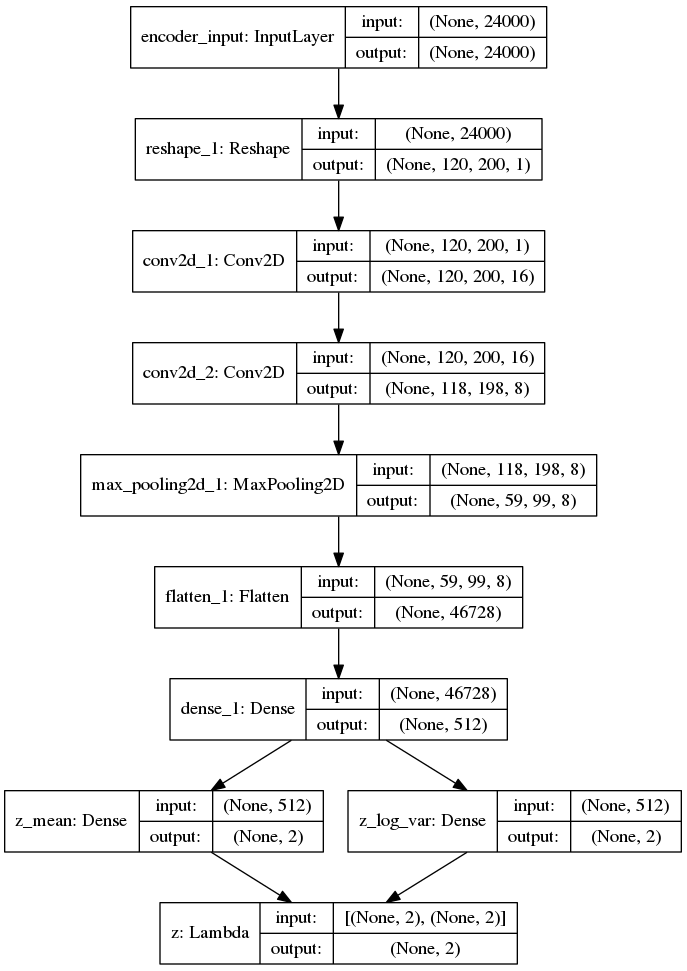
\includegraphics[width=1\linewidth]{vae_mlp_encoder}
		\caption{Convolutional encoder layers}
		\label{fig:encoder}
	\end{subfigure}
	\begin{subfigure}{.49\textwidth}
		\centering
		\begin{subfigure}{.6\textwidth}
			\centering
			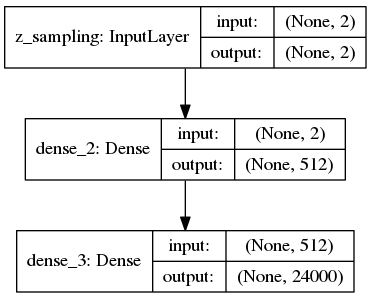
\includegraphics[width=1\linewidth]{vae_mlp_decoder}
			\caption{Decoder layers}
			\label{fig:vae_decoder}
		\end{subfigure}
		\vspace{10mm}%
		\begin{subfigure}{.8\textwidth}
			\centering
			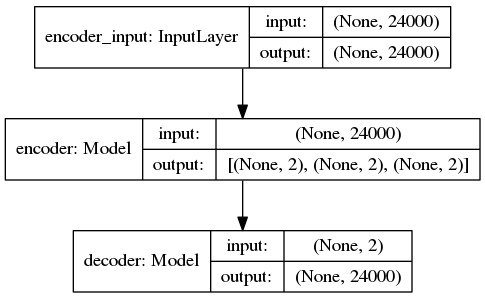
\includegraphics[width=1\linewidth]{vae_mlp}
			\caption{Combined model summary}
			\label{fig:vae_mlp}
		\end{subfigure}
		\label{fig:decoder}
	\end{subfigure}
	
	\caption{Layers of a Variational Autoencoder (VAE). The statistical values are at the end of the encoder in \ref{fig:encoder}, where the layers split into \texttt{z\_mean} and \texttt{z\_log\_var}. At those stages, a function is called that takes in the inputs from the previous \texttt{Dense} layer and encodes the information into two numbers using K-means functions provided by Keras. The output from the encoder, \texttt{z}, is what goes into the first layer of the decoder in \ref{fig:vae_decoder}. Additionally, the output \texttt{Dense()} layer in the decoder has the same size as the \texttt{InputLayer()} in \ref{fig:encoder}, clearly demonstrating the difference between a VAE and a supervised network, which outputs a class number rather than a decoded image.}
	\label{fig:vae}
\end{figure} 

The output of interest from the VAE is the statistical plot that can reveal clusters of data. Since training an unsupervised network does not depend on labels, the VAE can be run both without any assumed classes and with labels that we think correspond to clusters. Finding clusters is especially important for future sub-classification because if no clusters are found, it is likely to be extremely difficult for a neural network to distinguish between the different types of blips, no matter how easy it is for us to see the differences by eye. The next section goes through the clustering found by my VAE.

\subsubsection{Results of Unsupervised Network}

The first run of the VAE used no labels and included all the blips from both detectors during O2. Unsurprisingly, there are so many dots on the scatter plot that it is practically impossible to distinguish any patterns, let alone clear clusters, as seen in Figure \ref{fig:vae_unlabeled} on page \pageref{fig:unlabeled}. However, labeling each blip with its interferometer distinguishes the blips slightly more in Figure \ref{fig:vae_ifo_unlabeled}. Looking closer at these initial plots, the scatter plot of the unlabeled blips in Figure \ref{fig:vae_unlabeled} does have areas of higher concentration and lower concentration, despite the uniformity. There is also a small cluster to the bottom right, definitely separate from the majority. This small cluster is also present in Figure \ref{fig:vae_ifo_unlabeled}. The rest of the blips in the right scatter plot also provide evidence of clustering. There are more Livingston blips in the upper left of the plot and more Hanford blips in the middle right, and while there is a ton of overlap, this plot continues to show the difference between the Hanford and Livingston blips, as mentioned multiple times throughout this paper.

\begin{figure}[h!]
	\centering
	\begin{subfigure}{.49\textwidth}
		\centering
		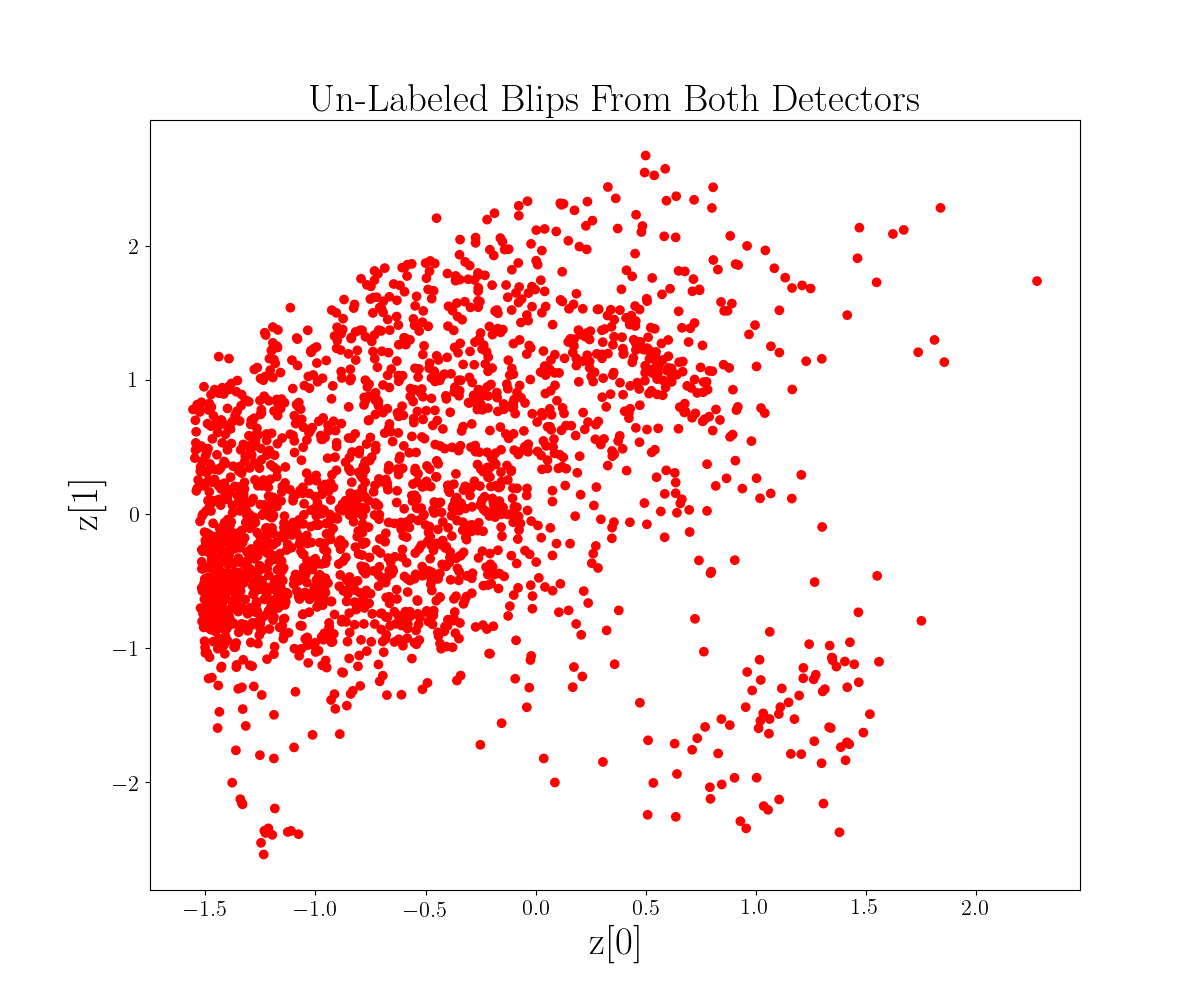
\includegraphics[width=1\linewidth]{vae_unlabeled}
		\caption{All blips from Hanford and Livingston}
		\label{fig:vae_unlabeled}
	\end{subfigure}
	\begin{subfigure}{.49\textwidth}
		\centering
		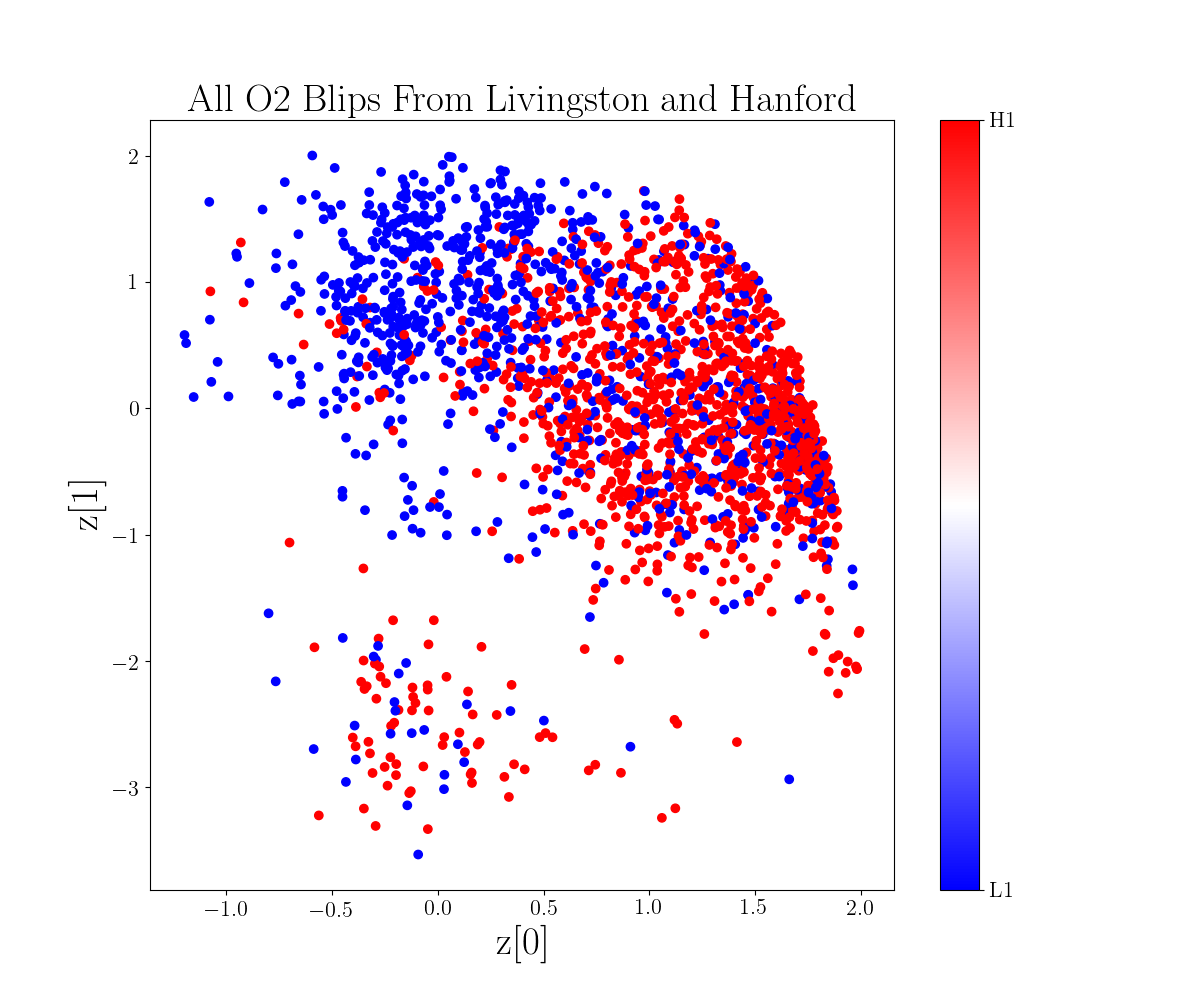
\includegraphics[width=1\linewidth]{vae_ifo_unlabeled}
		\caption{Blips labeled by interferometer}
		\label{fig:vae_ifo_unlabeled}
	\end{subfigure}
	\caption{Initial VAE scatter plots of all blips. The two axes are \texttt{z[0]} and \texttt{z[1]}, which are the output values from the K-means function called in the last layer of the encoder. The values themselves don't mean anything except in relation to each other. The overall shape and location of the dots are also arbitrary and change every time the neural network is run, but similar images will always map to similar \texttt{z[0]} and \texttt{z[1]} values. This is why the left plot has the majority of blips right by the y-axis but the right plot has them to the upper right.}
	\label{fig:unlabeled}
\end{figure}

Since there are considerably fewer images in the side cluster in Figure \ref{fig:unlabeled}, it is easy to look at the actual images in that cluster using saved data from when the VAE was trained and the scatter plot was created. The side cluster turns out to be images with indistinct signals, including spreads like those in section \ref{investigation} that were not resolved by the change in amount of data. The clustering of unresolved signals is actually a good sign for the validity of the VAE. Spreads and other unresolved signals look very different from their resolved counterparts, and this difference is clearly defined in the scatter plots. Interestingly, this discovery of spreads in my image database could also explain some of the troubles with the supervised neural networks, especially considering that my investigation at the beginning of section \ref{O2} found that spreading can happen to any type of blip. Unfortunately, since the reason for the spreading effect is still unknown, it is currently impossible to know how many of these images are in the image database and take them out of the image database without manually going through each of the 13,802 blip images. It is also fruitless to recreate the image database and re-train the neural networks without having a solid solution for the spreading. Based on the visual density of dots in Figures \ref{fig:vae_unlabeled} and \ref{fig:vae_ifo_unlabeled}, however, it is safe to say that the majority of blips have a resolved signal. The elimination of the unresolved signals would most likely allow for a clearer picture of other clusters, but for now we can simply ignore the side cluster. 

At the beginning of the discussion about neural networks in section \ref{section:build_nn}, I mentioned the lack of already-sub-classified blips as a reason why supervised learning may be ineffective in this project. By this point in the summer, however, I had labeled just over 2,000 of the 13,802 O2 blips, or about 15\%, all of which were created from a randomly-shuffled array of blip GPS times. There were enough other issues with the supervised learning networks besides data size, so I wanted to use these labeled blips in unsupervised learning instead. The labeled blips were taken out of the training set and set as the test images for the VAE. I trained my VAE on the other 85\% of the blips, and the resulting sub-class labeled scatter plot is in Figure \ref{fig:final_vae}. The scatter plot has clear, visible clusters! No colorbar can fully encapsulate seven different colors in a distinguishable way, so Figure \ref{fig:detailed_vae} on page \pageref{fig:detailed_vae} has some additional labels to help with seeing the different clusters and their corresponding sub-classes. 

\begin{figure}[h!]
	\centering
	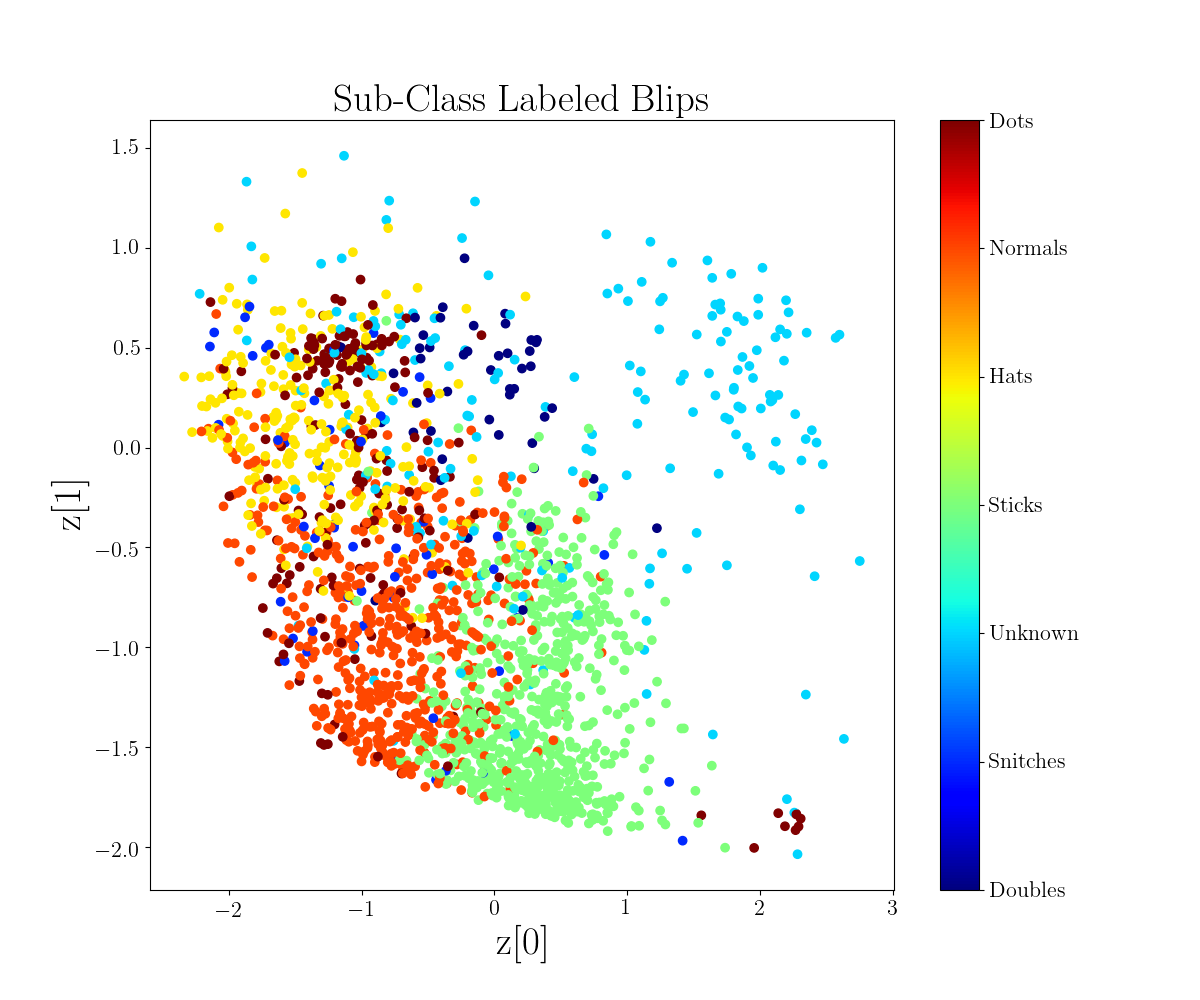
\includegraphics[width=.8\linewidth]{vae_test_labeled4}
	\caption{Sub-class labeled test blips.}
	\label{fig:final_vae}
\end{figure}

There are a bunch of important take-aways from this scatter plot. First and foremost, this plot demonstrates that a neural network can be built to distinguish certain sub-classes of blips. There is overlap between the clusters, but the hat cluster in the mid-to-upper left is independent of the stick cluster in the middle bottom of the plot, demonstrating definitive clustering. Second, we can easily distinguish the side cluster of unresolved signals, labeled here as unknowns. It is important that we didn't lose this cluster between runs of the neural network, otherwise we cannot trust these results. 

Third, we can clearly see that three of the types of blips make up the majority: hats, normals, and sticks. The images used to create this plot are a random representation of all blips, and while manual sub-classification did give me the impression that there are more hats, normals, and sticks compared to the other types of blips, the scatter plot provides compelling evidence. Knowing which types of blips are more frequent, and that they can be distinguished from each other, is important for prioritizing sub-classification in future work. Based on this scatter plot, LIGO could eliminate almost all blips from both detectors by eliminating hats, normals, and sticks. 

The more detailed plot in Figure \ref{fig:detailed_vae} brings another set of conclusions. The two most interesting things from the labels are the two completely separate clusters of dots and the lack of a snitch cluster. It is extremely unfortunate that the snitches did not cluster because their unique shape could make it easier to find its source compared to some of the other shapes. The lack of a cluster is probably because there are so few snitches overall. The fewer the images, the worse the neural network trains for that particular type of image. Additionally, the snitches could be clustered together and simply obscured by the multitude of other blips. 

\begin{figure}[h!]
	\centering
	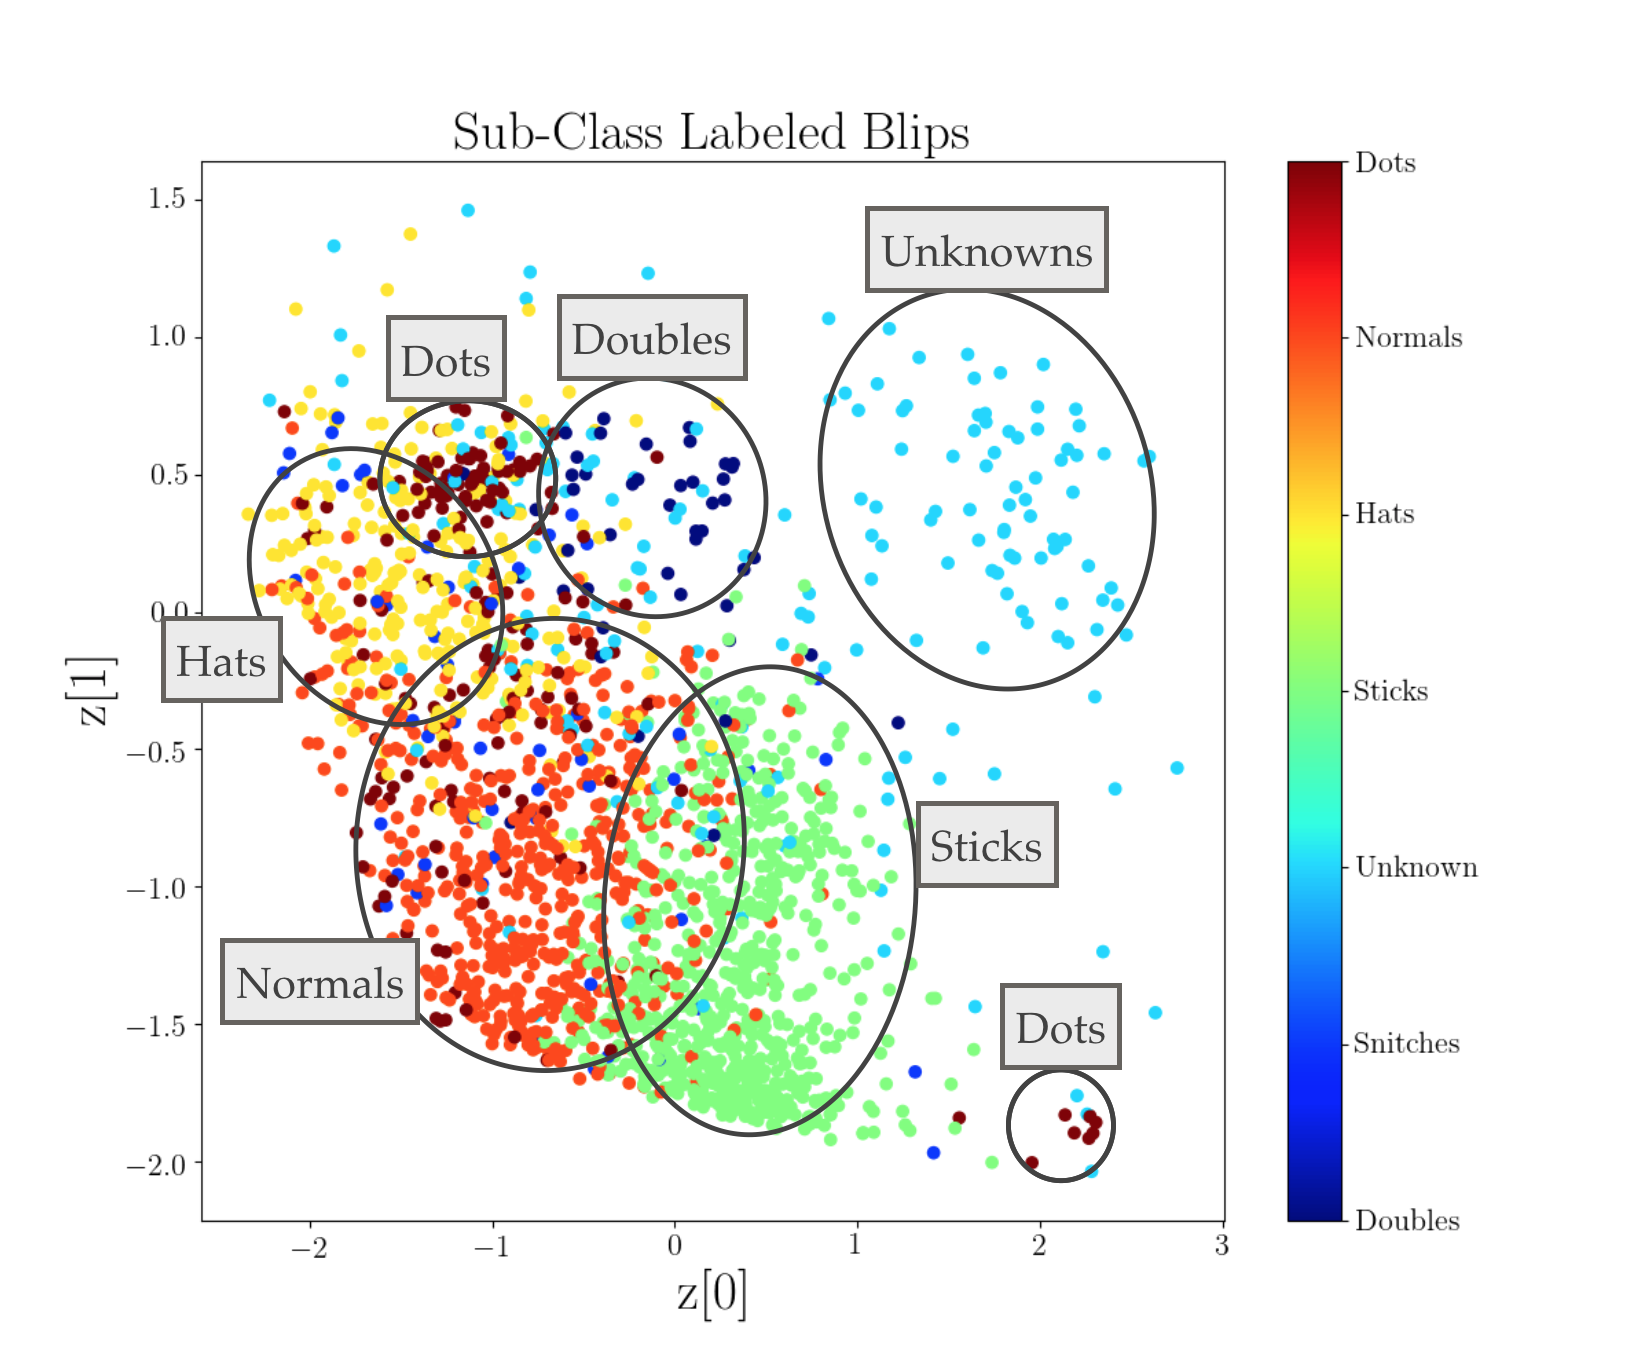
\includegraphics[width=.8\linewidth]{vae_detailed}
	\caption{Same scatter plot as Figure \ref{fig:final_vae}, with labels of clusters for more clarity. The snitches are the only sub-class that does not have its own separate cluster, and dots are the only sub-class that has multiple clusters.}
	\label{fig:detailed_vae}
\end{figure}

The two clusters of dot blips are both curious and informative. I labeled dots based on their round, circular shape, but the two clusters suggest two different sub-classes. I saved data about the GPS time, label, and coordinates for each blip on the scatter plot, and looking at the actual images from each cluster reveals the distinction, as shown in Figure \ref{fig:two_dots}. The left blip is from the upper left dot cluster and the right blip is from the bottom right cluster. While both blips have a round shape, the blips are at different frequencies and the right blip has a considerably higher energy. Based on the clustering in Figure \ref{fig:final_vae}, these two should be different sub-classes. I call the high-energy, high-frequency dot blips "suns," and stick to "dots" for the others.

\begin{figure}[h!]
	\centering
	\begin{subfigure}{.49\textwidth}
		\centering
		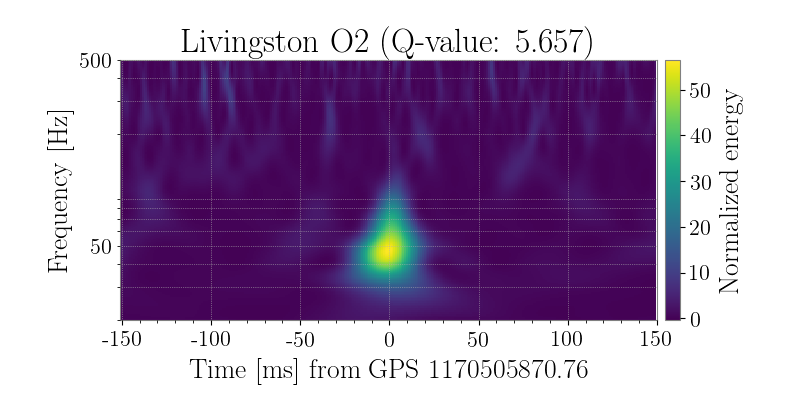
\includegraphics[width=1\linewidth]{dot_lowF}
		\caption{Dot blip from upper left cluster in Figure \ref{fig:detailed_vae}.}
		\label{fig:dot_lowf}
	\end{subfigure}
	\begin{subfigure}{.49\textwidth}
		\centering
		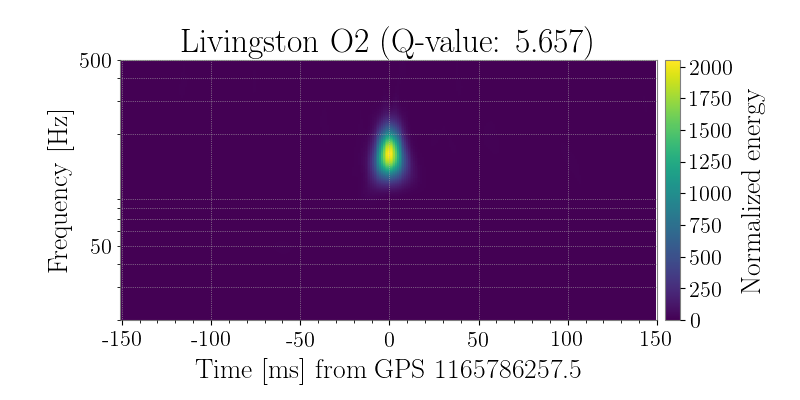
\includegraphics[width=1\linewidth]{dot_highF}
		\caption{Sun blip from upper left cluster in Figure \ref{fig:detailed_vae}.}
		\label{fig:dot_highf}
	\end{subfigure}
	\caption{Dot-labeled blips from VAE results. The shapes of the two blips are very similar, but the sun blip is at a different frequency and has a higher energy.}
	\label{fig:two_dots}
\end{figure}

Another important conclusion from Figures \ref{fig:final_vae} and \ref{fig:detailed_vae} is the overlap between the clusters. In particular, the normal cluster and the stick cluster are not only touching but intermixed. To investigate this result, I again used the data saved from the creation of the scatter plot to look at normals and sticks that clustered together. Figure \ref{fig:overlap} shows two blips within this overlap. The left blip was labeled as a normal and the right blip was labeled as a stick\textemdash the only visible difference between the two is that the "stick" trails upward past where the "normal" appears to end. Fortunately, these images explain why the VAE could not define clear clusters, but they leave the possibility of needing to add another sub-class. Creating another sub-class in between the normals and sticks is not as easy as adding sun blips, though, and doing so requires further attention and investigation.


\begin{figure}[h!]
	\centering
	\begin{subfigure}{.49\textwidth}
		\centering
		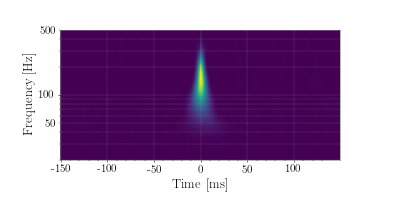
\includegraphics[width=1\linewidth]{normalish}
		\caption{Normal blip from overlap in Figure \ref{fig:detailed_vae}.}
		\label{fig:normalish}
	\end{subfigure}
	\begin{subfigure}{.49\textwidth}
		\centering
		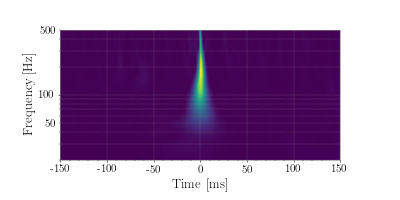
\includegraphics[width=1\linewidth]{stickish}
		\caption{Stick blip from overlap in Figure \ref{fig:detailed_vae}.}
		\label{fig:stickish}
	\end{subfigure}
	\caption{Two very similar-looking blips from the same region on the VAE scatter plot.}
	\label{fig:overlap}
\end{figure}



\section{Conclusions and Future Work}

Three of the different shapes of blips that I found in my initial investigation\textemdash hat, normal, and stick blips\textemdash were distinguishable from each other by the neural network. As described in the previous section, there is still work to be done to further define these sub-classes before moving forward with the larger goal of finding the sources of these blips, but the results of the unsupervised neural network established a real possibility of sub-classification of blip glitches. The other possible sub-classes each have their own potential and future work could improve their distinctions as well, as shown by the discovery of the sun blip within the dot blip sub-class. If the three frequent blips could be further distinguished from each other through information from unsupervised learning, the next step would be to sub-classify the rest of the blips using supervised learning and begin looking for sources of those three types of blips. 

The other area of future work is finding the cause of the spreading effect, which likely has something to do with the GWpy code and the whitening that occurs during a Q-transform calculation. If the spreading problem is eliminated, the other blips to look at are the double blips. I mentioned early on that the low-frequency signal inside the double blip might just be a whitening artifact, and an investigation into spreading might also result in a change to the spectrogram of the double-blips.

Another aspect that I did not get to explore is the energy differences between the blip images. The images put into the neural network all had different energies, mostly because the energies vary so much that a single normalized energy creates an over-saturated image for high-energy blips and a very dim outline for low-energy blips. One possibility for improving the neural network input is to use multiple images with different energy levels for each blip, similar to how GravitySpy uses multiple time domains for each glitch. This may help with defining more distinct sub-classes, an example of which is the sun blip I found from the VAE scatter plot. Multiple normalized energies make it clear that the dot blips and sun blips are different, even though their general shape is the same. Based on the late discovery of the sun blip, it might also be worth manually exploring blips again, this time using images of different normalized energy. There is a strong possibility that more than one of the six initial spectrogram shapes could be split into multiple subclasses through relative energy. 

The results presented in this paper provided ample evidence that the goal of sub-classification of blips is attainable. If the sub-classifications of blips found in this project become even more distinguishable in the VAE by altering labels and inputs, we can go back to supervised learning and start to sub-classify the rest of the thousands of blips from O2, bringing us closer to the goal of finding the sources of the blips and eliminating them from the detectors. 

\bibliography{references}
\bibliographystyle{ieeetr}

\end{document}

































